\documentclass[14pt,ignorenonframetext,]{beamer}
\setbeamertemplate{caption}[numbered]
\setbeamertemplate{caption label separator}{: }
\setbeamercolor{caption name}{fg=normal text.fg}
\beamertemplatenavigationsymbolsempty
\usepackage{lmodern}
\usepackage{amssymb,amsmath}
\usepackage{ifxetex,ifluatex}
\usepackage{fixltx2e} % provides \textsubscript
\ifnum 0\ifxetex 1\fi\ifluatex 1\fi=0 % if pdftex
  \usepackage[T1]{fontenc}
  \usepackage[utf8]{inputenc}
\else % if luatex or xelatex
  \ifxetex
    \usepackage{mathspec}
  \else
    \usepackage{fontspec}
  \fi
  \defaultfontfeatures{Ligatures=TeX,Scale=MatchLowercase}
\fi
\usetheme[]{metropolis}
% use upquote if available, for straight quotes in verbatim environments
\IfFileExists{upquote.sty}{\usepackage{upquote}}{}
% use microtype if available
\IfFileExists{microtype.sty}{%
\usepackage{microtype}
\UseMicrotypeSet[protrusion]{basicmath} % disable protrusion for tt fonts
}{}
\newif\ifbibliography
\hypersetup{
            pdftitle={BIA6315},
            pdfauthor={Ch8. ARIMA models},
            pdfborder={0 0 0},
            breaklinks=true}
\urlstyle{same}  % don't use monospace font for urls
\usepackage{color}
\usepackage{fancyvrb}
\newcommand{\VerbBar}{|}
\newcommand{\VERB}{\Verb[commandchars=\\\{\}]}
\DefineVerbatimEnvironment{Highlighting}{Verbatim}{commandchars=\\\{\}}
% Add ',fontsize=\small' for more characters per line
\usepackage{framed}
\definecolor{shadecolor}{RGB}{248,248,248}
\newenvironment{Shaded}{\begin{snugshade}}{\end{snugshade}}
\newcommand{\KeywordTok}[1]{\textcolor[rgb]{0.13,0.29,0.53}{\textbf{#1}}}
\newcommand{\DataTypeTok}[1]{\textcolor[rgb]{0.13,0.29,0.53}{#1}}
\newcommand{\DecValTok}[1]{\textcolor[rgb]{0.00,0.00,0.81}{#1}}
\newcommand{\BaseNTok}[1]{\textcolor[rgb]{0.00,0.00,0.81}{#1}}
\newcommand{\FloatTok}[1]{\textcolor[rgb]{0.00,0.00,0.81}{#1}}
\newcommand{\ConstantTok}[1]{\textcolor[rgb]{0.00,0.00,0.00}{#1}}
\newcommand{\CharTok}[1]{\textcolor[rgb]{0.31,0.60,0.02}{#1}}
\newcommand{\SpecialCharTok}[1]{\textcolor[rgb]{0.00,0.00,0.00}{#1}}
\newcommand{\StringTok}[1]{\textcolor[rgb]{0.31,0.60,0.02}{#1}}
\newcommand{\VerbatimStringTok}[1]{\textcolor[rgb]{0.31,0.60,0.02}{#1}}
\newcommand{\SpecialStringTok}[1]{\textcolor[rgb]{0.31,0.60,0.02}{#1}}
\newcommand{\ImportTok}[1]{#1}
\newcommand{\CommentTok}[1]{\textcolor[rgb]{0.56,0.35,0.01}{\textit{#1}}}
\newcommand{\DocumentationTok}[1]{\textcolor[rgb]{0.56,0.35,0.01}{\textbf{\textit{#1}}}}
\newcommand{\AnnotationTok}[1]{\textcolor[rgb]{0.56,0.35,0.01}{\textbf{\textit{#1}}}}
\newcommand{\CommentVarTok}[1]{\textcolor[rgb]{0.56,0.35,0.01}{\textbf{\textit{#1}}}}
\newcommand{\OtherTok}[1]{\textcolor[rgb]{0.56,0.35,0.01}{#1}}
\newcommand{\FunctionTok}[1]{\textcolor[rgb]{0.00,0.00,0.00}{#1}}
\newcommand{\VariableTok}[1]{\textcolor[rgb]{0.00,0.00,0.00}{#1}}
\newcommand{\ControlFlowTok}[1]{\textcolor[rgb]{0.13,0.29,0.53}{\textbf{#1}}}
\newcommand{\OperatorTok}[1]{\textcolor[rgb]{0.81,0.36,0.00}{\textbf{#1}}}
\newcommand{\BuiltInTok}[1]{#1}
\newcommand{\ExtensionTok}[1]{#1}
\newcommand{\PreprocessorTok}[1]{\textcolor[rgb]{0.56,0.35,0.01}{\textit{#1}}}
\newcommand{\AttributeTok}[1]{\textcolor[rgb]{0.77,0.63,0.00}{#1}}
\newcommand{\RegionMarkerTok}[1]{#1}
\newcommand{\InformationTok}[1]{\textcolor[rgb]{0.56,0.35,0.01}{\textbf{\textit{#1}}}}
\newcommand{\WarningTok}[1]{\textcolor[rgb]{0.56,0.35,0.01}{\textbf{\textit{#1}}}}
\newcommand{\AlertTok}[1]{\textcolor[rgb]{0.94,0.16,0.16}{#1}}
\newcommand{\ErrorTok}[1]{\textcolor[rgb]{0.64,0.00,0.00}{\textbf{#1}}}
\newcommand{\NormalTok}[1]{#1}
\usepackage{longtable,booktabs}
\usepackage{caption}
% These lines are needed to make table captions work with longtable:
\makeatletter
\def\fnum@table{\tablename~\thetable}
\makeatother
\usepackage{graphicx,grffile}
\makeatletter
\def\maxwidth{\ifdim\Gin@nat@width>\linewidth\linewidth\else\Gin@nat@width\fi}
\def\maxheight{\ifdim\Gin@nat@height>\textheight0.8\textheight\else\Gin@nat@height\fi}
\makeatother
% Scale images if necessary, so that they will not overflow the page
% margins by default, and it is still possible to overwrite the defaults
% using explicit options in \includegraphics[width, height, ...]{}
\setkeys{Gin}{width=\maxwidth,height=\maxheight,keepaspectratio}

% Prevent slide breaks in the middle of a paragraph:
\widowpenalties 1 10000
\raggedbottom

\AtBeginPart{
  \let\insertpartnumber\relax
  \let\partname\relax
  \frame{\partpage}
}
\AtBeginSection{
  \ifbibliography
  \else
    \let\insertsectionnumber\relax
    \let\sectionname\relax
    \frame{\sectionpage}
  \fi
}
\AtBeginSubsection{
  \let\insertsubsectionnumber\relax
  \let\subsectionname\relax
  \frame{\subsectionpage}
}

\setlength{\parindent}{0pt}
\setlength{\parskip}{6pt plus 2pt minus 1pt}
\setlength{\emergencystretch}{3em}  % prevent overfull lines
\providecommand{\tightlist}{%
  \setlength{\itemsep}{0pt}\setlength{\parskip}{0pt}}
\setcounter{secnumdepth}{0}

\title{BIA6315}
\author{Ch8. ARIMA models}
\date{OTexts.org/fpp2/}

\begin{document}
\frame{\titlepage}

\section{Stationarity and
differencing}\label{stationarity-and-differencing}

\begin{frame}{Stationarity}

\begin{block}{Definition}
If $\{y_t\}$ is a stationary time series, then for all $s$, the distribution of $(y_t,\dots,y_{t+s})$ does not depend on $t$.
\end{block}

\pause

A \textbf{stationary series} is:

\begin{itemize}
\tightlist
\item
  roughly horizontal
\item
  constant variance
\item
  no patterns predictable in the long-term
\end{itemize}

\end{frame}

\begin{frame}{Stationary?}

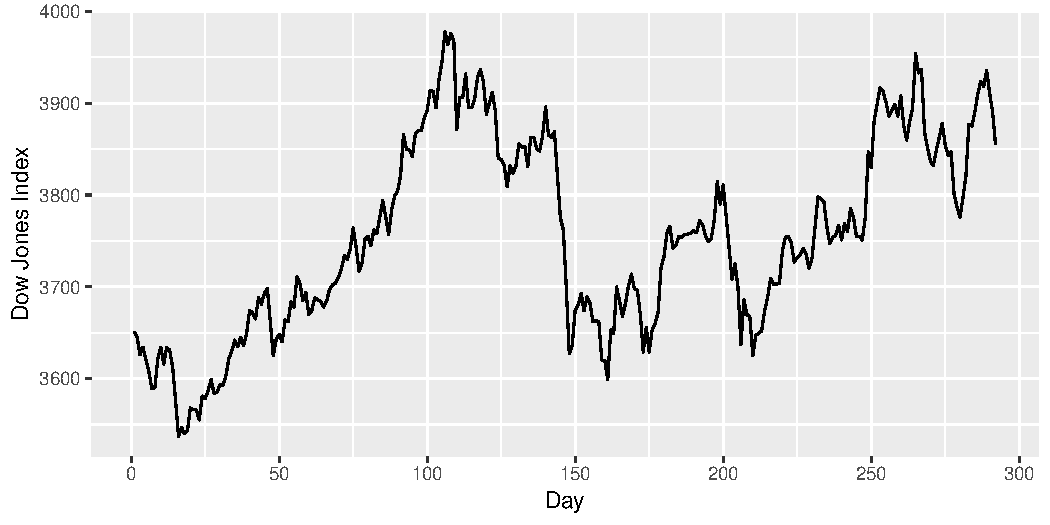
\includegraphics{week_5_arima_files/figure-beamer/unnamed-chunk-1-1.pdf}

\end{frame}

\begin{frame}{Stationary?}

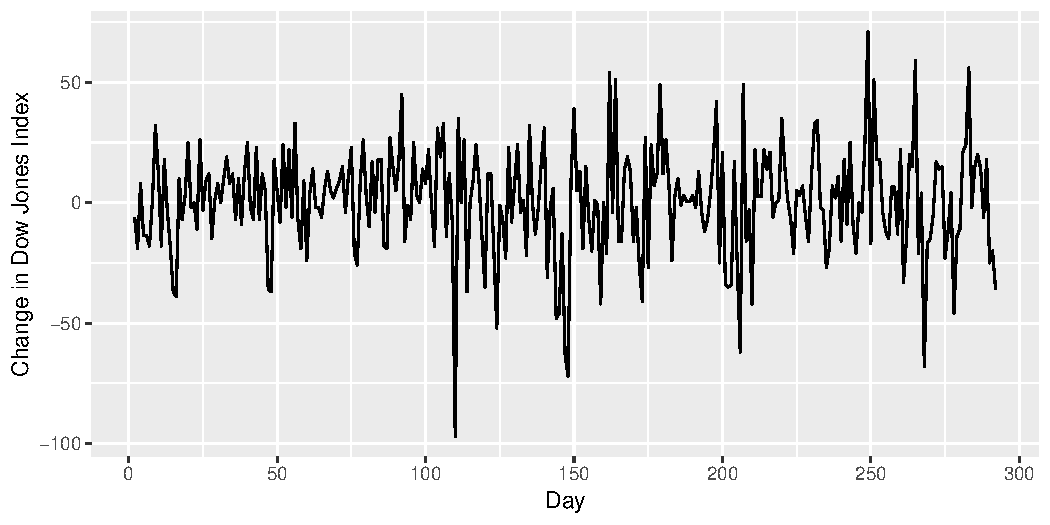
\includegraphics{week_5_arima_files/figure-beamer/unnamed-chunk-2-1.pdf}

\end{frame}

\begin{frame}{Stationary?}

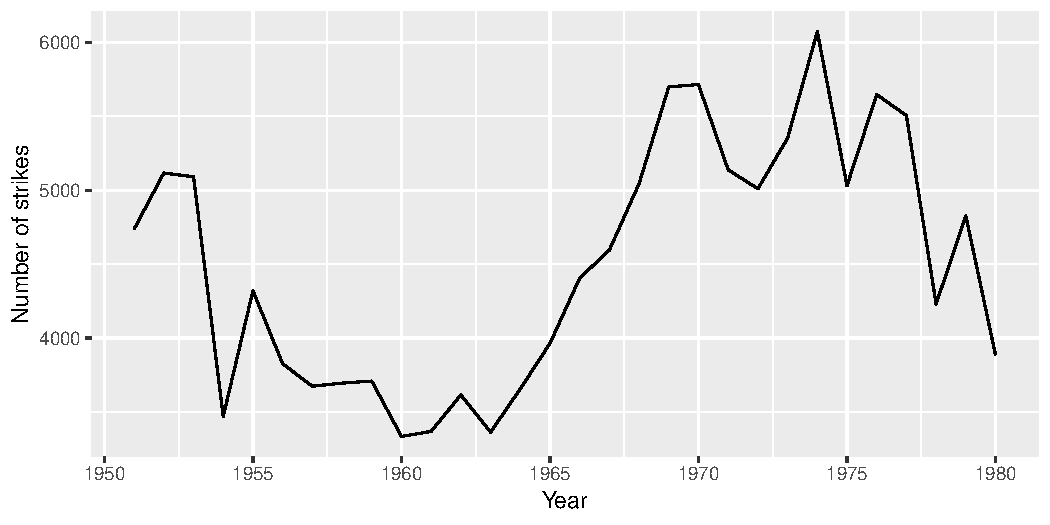
\includegraphics{week_5_arima_files/figure-beamer/unnamed-chunk-3-1.pdf}

\end{frame}

\begin{frame}{Stationary?}

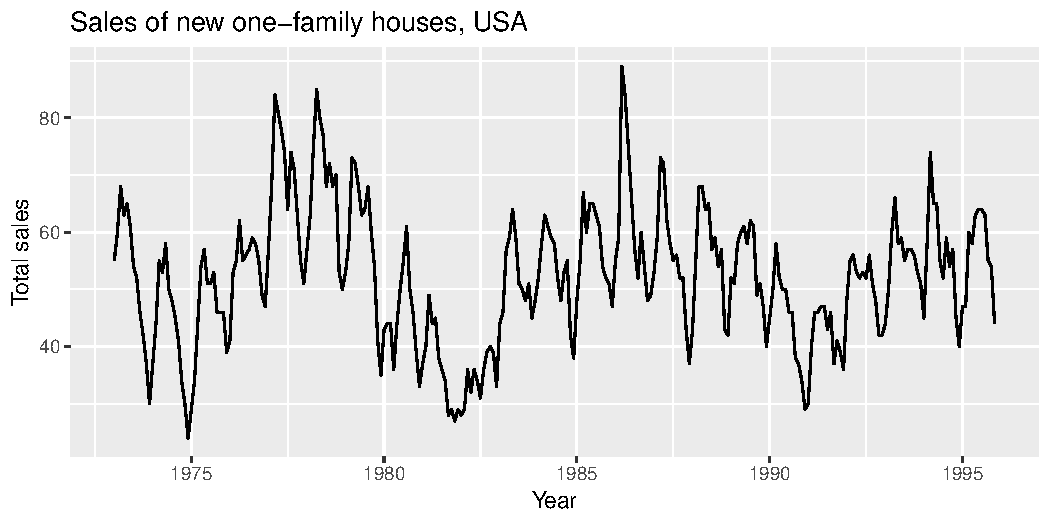
\includegraphics{week_5_arima_files/figure-beamer/unnamed-chunk-4-1.pdf}

\end{frame}

\begin{frame}{Stationary?}

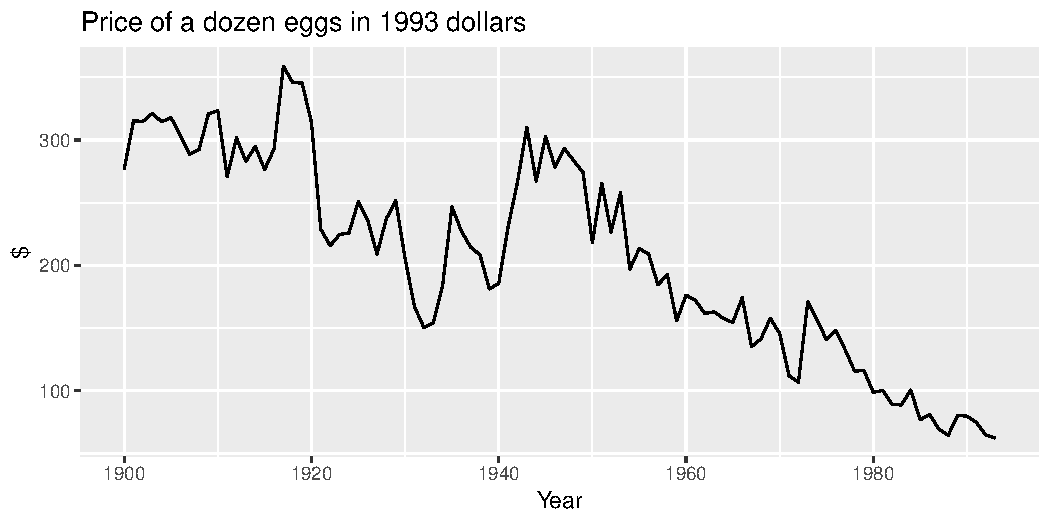
\includegraphics{week_5_arima_files/figure-beamer/unnamed-chunk-5-1.pdf}

\end{frame}

\begin{frame}{Stationary?}

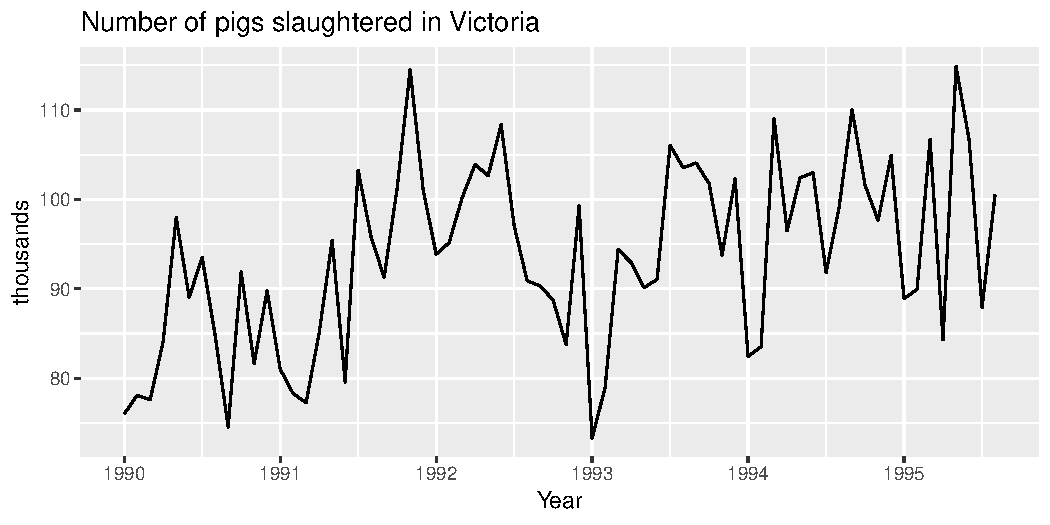
\includegraphics{week_5_arima_files/figure-beamer/unnamed-chunk-6-1.pdf}

\end{frame}

\begin{frame}{Stationary?}

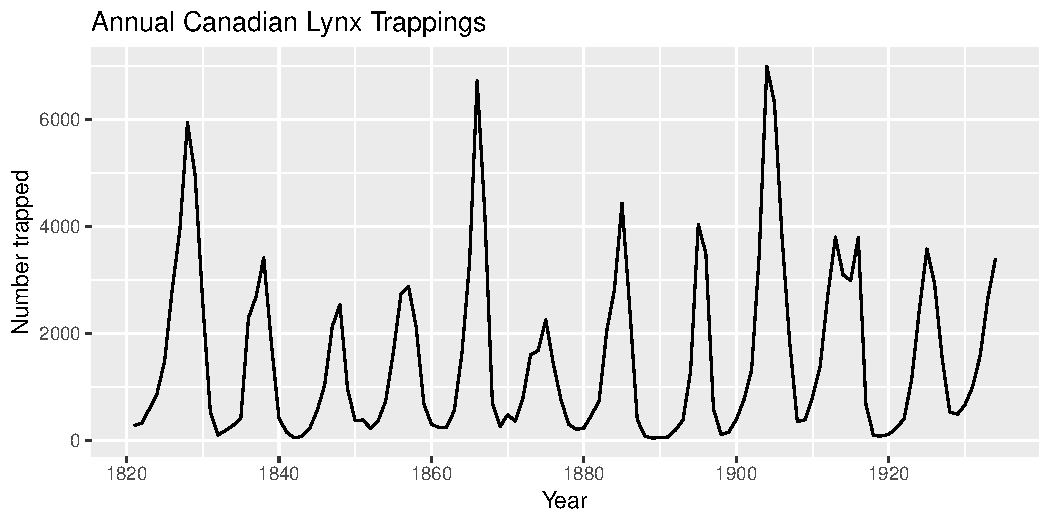
\includegraphics{week_5_arima_files/figure-beamer/unnamed-chunk-7-1.pdf}

\end{frame}

\begin{frame}{Stationary?}

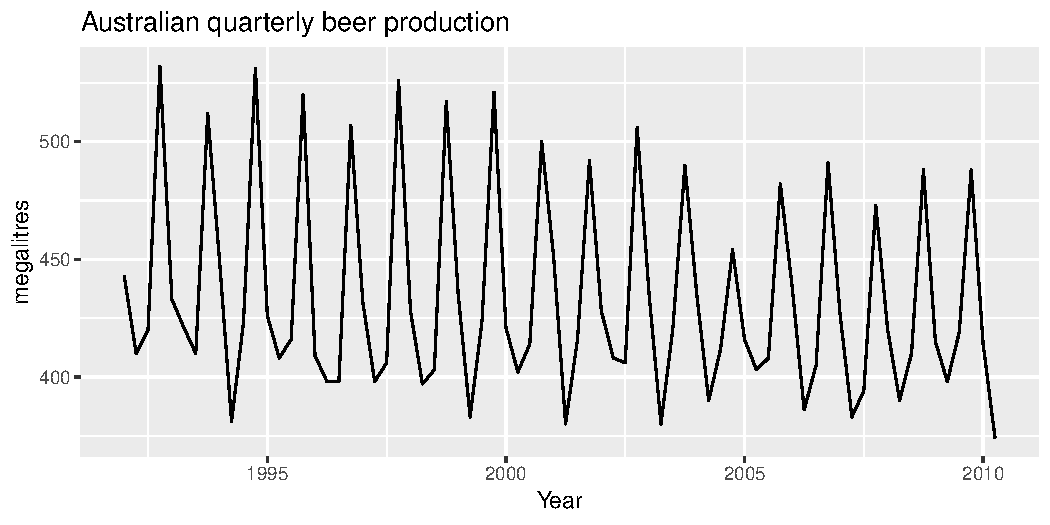
\includegraphics{week_5_arima_files/figure-beamer/unnamed-chunk-8-1.pdf}

\end{frame}

\begin{frame}{Stationarity}

\begin{block}{Definition}
If $\{y_t\}$ is a stationary time series, then for all $s$, the distribution of $(y_t,\dots,y_{t+s})$ does not depend on $t$.
\end{block}

\pause\vspace*{0.4cm}

Transformations help to \textbf{stabilize the variance}.

For ARIMA modelling, we also need to \textbf{stabilize the mean}.

\end{frame}

\begin{frame}{Non-stationarity in the mean}

\structure{Identifying non-stationary series}

\begin{itemize}
\item
  time plot.
\item
  The ACF of stationary data drops to zero relatively quickly
\item
  The ACF of non-stationary data decreases slowly.
\item
  For non-stationary data, the value of \(r_1\) is often large and
  positive.
\end{itemize}

\end{frame}

\begin{frame}{Example: Dow-Jones index}

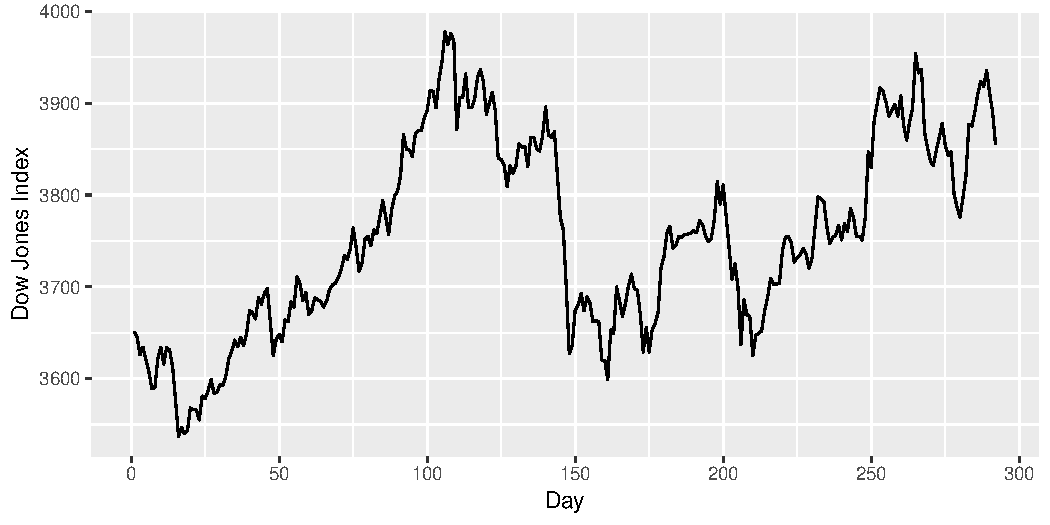
\includegraphics{week_5_arima_files/figure-beamer/unnamed-chunk-9-1.pdf}

\end{frame}

\begin{frame}{Example: Dow-Jones index}

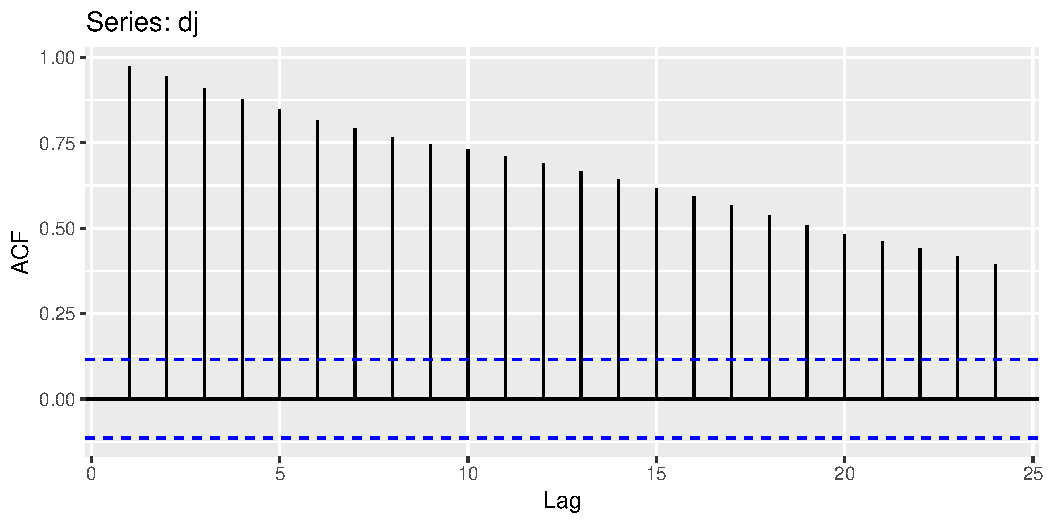
\includegraphics{week_5_arima_files/figure-beamer/unnamed-chunk-10-1.pdf}

\end{frame}

\begin{frame}{Example: Dow-Jones index}

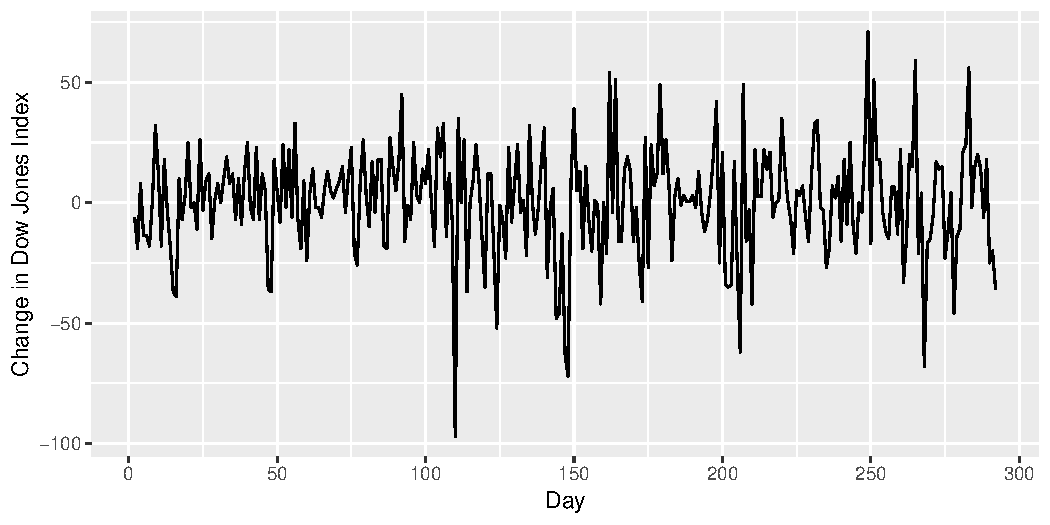
\includegraphics{week_5_arima_files/figure-beamer/unnamed-chunk-11-1.pdf}

\end{frame}

\begin{frame}{Example: Dow-Jones index}

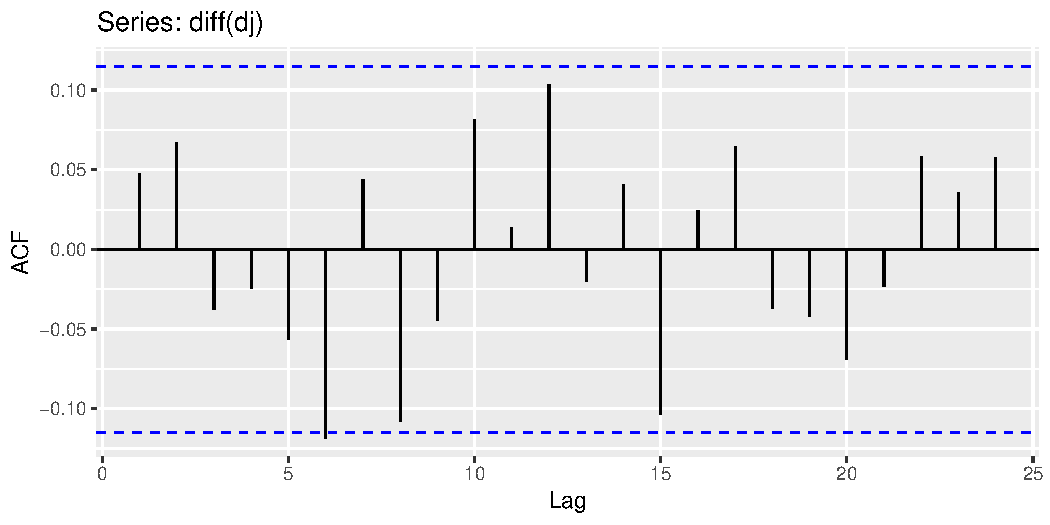
\includegraphics{week_5_arima_files/figure-beamer/unnamed-chunk-12-1.pdf}

\end{frame}

\begin{frame}{Differencing}

\begin{itemize}
\tightlist
\item
  Differencing helps to \textbf{stabilize the mean}.
\item
  The differenced series is the \emph{change} between each observation
  in the original series: \({y'_t = y_t - y_{t-1}}\).
\item
  The differenced series will have only \(T-1\) values since it is not
  possible to calculate a difference \(y_1'\) for the first observation.
\end{itemize}

\end{frame}

\begin{frame}{Second-order differencing}

Occasionally the differenced data will not appear stationary and it may
be necessary to difference the data a second time:\pause

\begin{align*}
y''_{t}  &=  y'_{t}  - y'_{t - 1} \\
&= (y_t - y_{t-1}) - (y_{t-1}-y_{t-2})\\
&= y_t - 2y_{t-1} +y_{t-2}.
\end{align*}

\pause

\begin{itemize}
\tightlist
\item
  \(y_t''\) will have \(T-2\) values.
\item
  In practice, it is almost never necessary to go beyond second-order
  differences.
\end{itemize}

\end{frame}

\begin{frame}{Seasonal differencing}

A seasonal difference is the difference between an observation and the
corresponding observation from the previous year.\pause
\[{y'_t = y_t - y_{t-m}}\] where \(m=\) number of seasons.\pause

\begin{itemize}
\tightlist
\item
  For monthly data \(m=12\).
\item
  For quarterly data \(m=4\).
\end{itemize}

\end{frame}

\begin{frame}[fragile]{Electricity production}

\begin{Shaded}
\begin{Highlighting}[]
\NormalTok{usmelec }\OperatorTok\StringTok{ }\KeywordTok{autoplot}\NormalTok{()}
\end{Highlighting}
\end{Shaded}

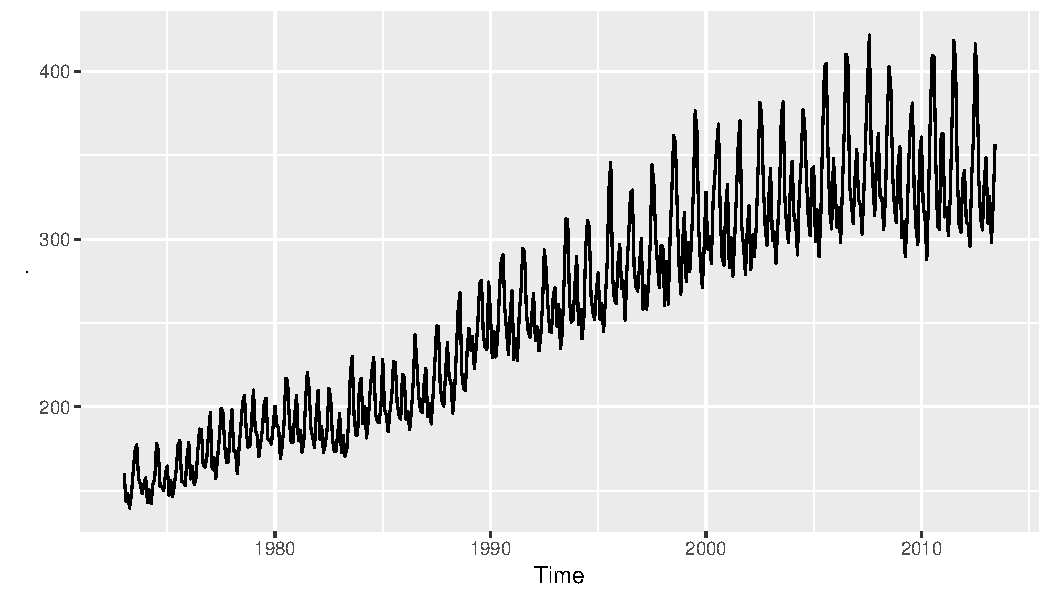
\includegraphics{week_5_arima_files/figure-beamer/unnamed-chunk-13-1.pdf}

\end{frame}

\begin{frame}[fragile]{Electricity production}

\begin{Shaded}
\begin{Highlighting}[]
\NormalTok{usmelec }\OperatorTok\StringTok{ }\KeywordTok{log}\NormalTok{() }\OperatorTok\StringTok{ }\KeywordTok{autoplot}\NormalTok{()}
\end{Highlighting}
\end{Shaded}

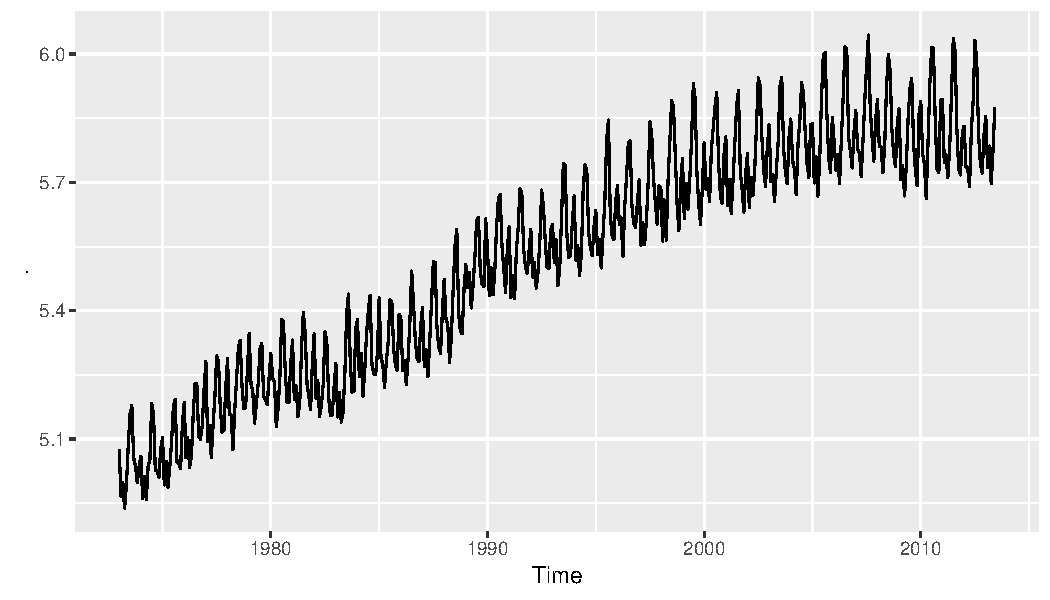
\includegraphics{week_5_arima_files/figure-beamer/unnamed-chunk-14-1.pdf}

\end{frame}

\begin{frame}[fragile]{Electricity production}

\begin{Shaded}
\begin{Highlighting}[]
\NormalTok{usmelec }\OperatorTok\StringTok{ }\KeywordTok{log}\NormalTok{() }\OperatorTok\StringTok{ }\KeywordTok{diff}\NormalTok{(}\DataTypeTok{lag=}\DecValTok{12}\NormalTok{) }\OperatorTok
\StringTok{  }\KeywordTok{autoplot}\NormalTok{()}
\end{Highlighting}
\end{Shaded}

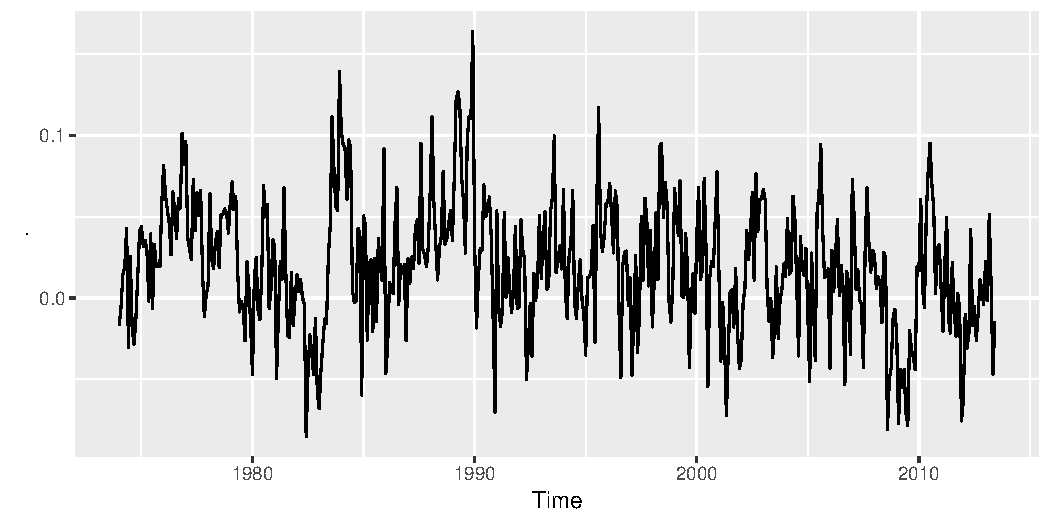
\includegraphics{week_5_arima_files/figure-beamer/unnamed-chunk-15-1.pdf}

\end{frame}

\begin{frame}[fragile]{Electricity production}

\begin{Shaded}
\begin{Highlighting}[]
\NormalTok{usmelec }\OperatorTok\StringTok{ }\KeywordTok{log}\NormalTok{() }\OperatorTok\StringTok{ }\KeywordTok{diff}\NormalTok{(}\DataTypeTok{lag=}\DecValTok{12}\NormalTok{) }\OperatorTok
\StringTok{  }\KeywordTok{diff}\NormalTok{(}\DataTypeTok{lag=}\DecValTok{1}\NormalTok{) }\OperatorTok\StringTok{ }\KeywordTok{autoplot}\NormalTok{()}
\end{Highlighting}
\end{Shaded}

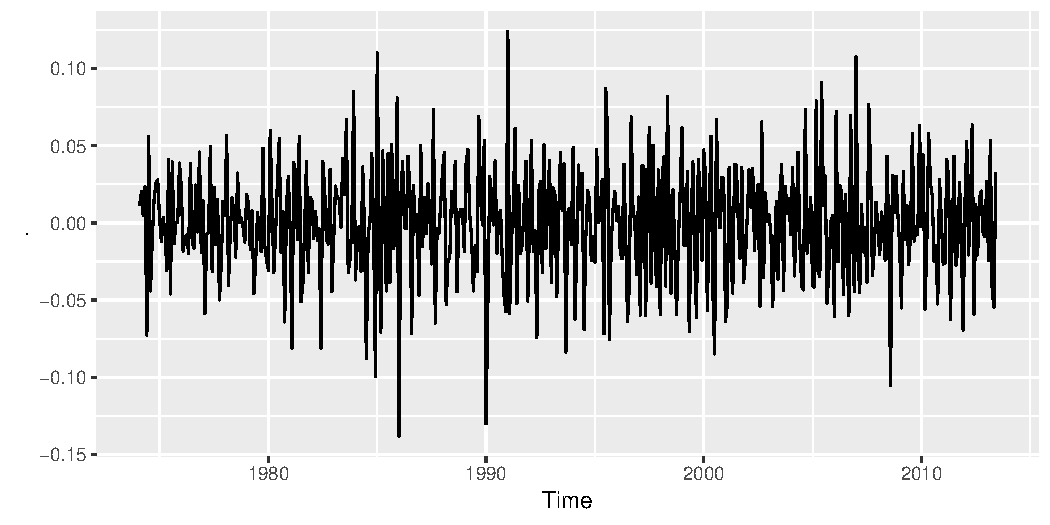
\includegraphics{week_5_arima_files/figure-beamer/unnamed-chunk-16-1.pdf}

\end{frame}

\begin{frame}{Electricity production}

\begin{itemize}
\tightlist
\item
  Seasonally differenced series is closer to being stationary.
\item
  Remaining non-stationarity can be removed with further first
  difference.
\end{itemize}

If \(y'_t = y_t - y_{t-12}\) denotes seasonally differenced series, then
twice-differenced series i

\begin{block}{}
\begin{align*}
y^*_t &= y'_t - y'_{t-1} \\
      &= (y_t - y_{t-12}) - (y_{t-1} - y_{t-13}) \\
      &= y_t - y_{t-1} - y_{t-12} + y_{t-13}\: .
\end{align*}
\end{block}

\vspace*{10cm}

\end{frame}

\begin{frame}{Seasonal differencing}

When both seasonal and first differences are applied\dots\pause

\begin{itemize}
\tightlist
\item
  it makes no difference which is done first---the result will be the
  same.
\item
  If seasonality is strong, we recommend that seasonal differencing be
  done first because sometimes the resulting series will be stationary
  and there will be no need for further first difference. \pause
\end{itemize}

It is important that if differencing is used, the differences are
interpretable.

\end{frame}

\begin{frame}{Interpretation of differencing}

\begin{itemize}
\tightlist
\item
  first differences are the change between
  \textbf{one observation and the
  next};
\item
  seasonal differences are the change between \textbf{one year to the
  next}. \pause
\end{itemize}

But taking lag 3 differences for yearly data, for example, results in a
model which cannot be sensibly interpreted.

\end{frame}

\begin{frame}{Unit root tests}

\structure{Statistical tests to determine the required order of differencing.}

\begin{enumerate}
\def\labelenumi{\arabic{enumi}.}
\tightlist
\item
  Augmented Dickey Fuller test: null hypothesis is that the data are
  non-stationary and non-seasonal.
\item
  Kwiatkowski-Phillips-Schmidt-Shin (KPSS) test: null hypothesis is that
  the data are stationary and non-seasonal.
\item
  Other tests available for seasonal data.
\end{enumerate}

\end{frame}

\begin{frame}[fragile]{KPSS test}

\fontsize{10}{11}\sf

\begin{Shaded}
\begin{Highlighting}[]
\KeywordTok{library}\NormalTok{(urca)}
\KeywordTok{summary}\NormalTok{(}\KeywordTok{ur.kpss}\NormalTok{(goog))}
\end{Highlighting}
\end{Shaded}

\begin{verbatim}
## 
## ####################### 
## # KPSS Unit Root Test # 
## ####################### 
## 
## Test is of type: mu with 7 lags. 
## 
## Value of test-statistic is: 10.7223 
## 
## Critical value for a significance level of: 
##                 10pct  5pct 2.5pct  1pct
## critical values 0.347 0.463  0.574 0.739
\end{verbatim}

\pause

\begin{Shaded}
\begin{Highlighting}[]
\KeywordTok{ndiffs}\NormalTok{(goog)}
\end{Highlighting}
\end{Shaded}

\begin{verbatim}
## [1] 1
\end{verbatim}

\end{frame}

\begin{frame}[fragile]{Automatically selecting differences}

STL decomposition: \(y_t = T_t+S_t+R_t\)

Seasonal strength
\(F_s = \max\big(0, 1-\frac{\text{Var}(R_t)}{\text{Var}(S_t+R_t)}\big)\)

If \(F_s > 0.64\), do one seasonal difference.

\pause\fontsize{12}{15}\sf\vspace*{1cm}

\begin{Shaded}
\begin{Highlighting}[]
\NormalTok{usmelec }\OperatorTok\StringTok{ }\KeywordTok{log}\NormalTok{() }\OperatorTok\StringTok{ }\KeywordTok{nsdiffs}\NormalTok{()}
\end{Highlighting}
\end{Shaded}

\begin{verbatim}
## [1] 1
\end{verbatim}

\begin{Shaded}
\begin{Highlighting}[]
\NormalTok{usmelec }\OperatorTok\StringTok{ }\KeywordTok{log}\NormalTok{() }\OperatorTok\StringTok{ }\KeywordTok{diff}\NormalTok{(}\DataTypeTok{lag=}\DecValTok{12}\NormalTok{) }\OperatorTok\StringTok{ }\KeywordTok{ndiffs}\NormalTok{()}
\end{Highlighting}
\end{Shaded}

\begin{verbatim}
## [1] 1
\end{verbatim}

\end{frame}

\begin{frame}[fragile]{Your turn}

For the \texttt{visitors} series, find an appropriate differencing
(after transformation if necessary) to obtain stationary data.

\end{frame}

\begin{frame}{Backshift notation}

A very useful notational device is the backward shift operator, \(B\),
which is used as follows: \[
{B y_{t}  =  y_{t - 1}} \: .
\]\pause
In other words, \(B\), operating on \(y_{t}\), has the effect of
\textbf{shifting  the  data  back  one   period}. \pause
Two applications of \(B\) to \(y_{t}\)
\textbf{shifts the data  back  two
periods}: \[
B(By_{t})  =  B^{2}y_{t}  =  y_{t-2}\: .
\]\pause
For monthly data, if we wish to shift attention to ``the same month last
year,'' then \(B^{12}\) is used, and the notation is \(B^{12}y_{t}\) =
\(y_{t-12}\).

\end{frame}

\begin{frame}{Backshift notation}

The backward shift operator is convenient for describing the process of
\textit{differencing}. \pause
A first difference can be written as \[
y'_{t}  =  y_{t} -   y_{t-1} = y_t - By_{t}  =  (1 - B)y_{t}\: .
\]\pause
Note that a first difference is represented by \((1 - B)\). \pause

Similarly, if second-order differences (i.e., first differences of first
differences) have to be computed, then: \[
y''_{t}  =  y_{t} -   2y_{t - 1}  +  y_{t - 2} = (1 - B)^{2} y_{t}\: .
\]

\end{frame}

\begin{frame}{Backshift notation}

\begin{itemize}
\item
  Second-order difference is denoted \((1- B)^{2}\).
\item
  \textit{Second-order  difference} is not the same as a
  \textit{second  difference}, which would be denoted \(1- B^{2}\);
\item
  In general, a \(d\)th-order difference can be written as
  \[(1 - B)^{d} y_{t}.\]
\item
  A seasonal difference followed by a first difference can be written as
  \[ (1-B)(1-B^m)y_t\: .\]
\end{itemize}

\end{frame}

\begin{frame}{Backshift notation}

The ``backshift'' notation is convenient because the terms can be
multiplied together to see the combined effect.

\begin{align*}
(1-B)(1-B^m)y_t &= (1 - B - B^m + B^{m+1})y_t \\
&= y_t-y_{t-1}-y_{t-m}+y_{t-m-1}.
\end{align*}

\pause
For monthly data, \(m=12\) and we obtain the same result as earlier.

\end{frame}

\section{Non-seasonal ARIMA models}\label{non-seasonal-arima-models}

\begin{frame}{Autoregressive models}

\begin{block}{Autoregressive (AR) models:}
$$
  y_{t}  =  c  +  \phi_{1}y_{t - 1}  +  \phi_{2}y_{t - 2}  +  \cdots  +  \phi_{p}y_{t - p}  + \varepsilon_{t},
$$
where $\varepsilon_t$ is white noise.  This is a multiple regression with \textbf{lagged values} of $y_t$ as predictors.
\end{block}

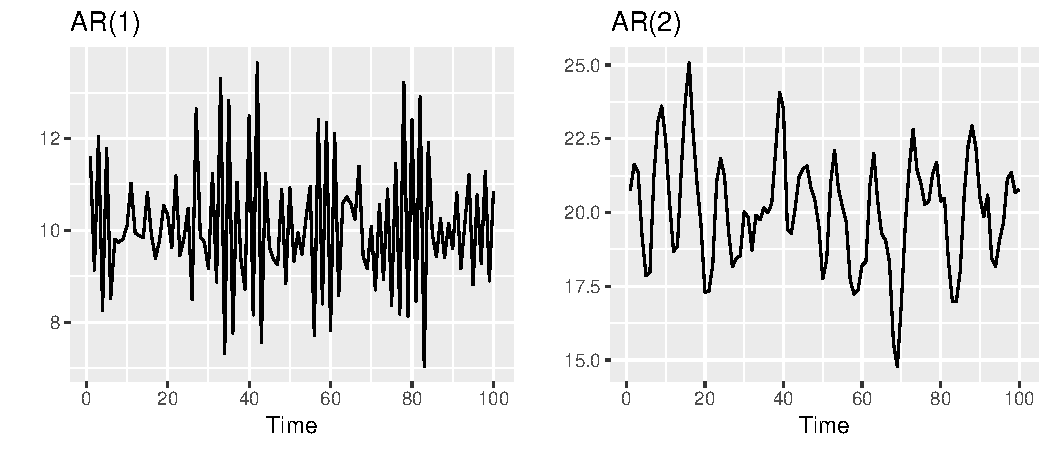
\includegraphics{week_5_arima_files/figure-beamer/arp-1.pdf}

\end{frame}

\begin{frame}{AR(1) model}

\begin{block}{}
\centerline{$y_{t}    =   2 -0.8 y_{t - 1}  +  \varepsilon_{t}$}
\end{block}

\rightline{$\varepsilon_t\sim N(0,1)$,\quad $T=100$.}

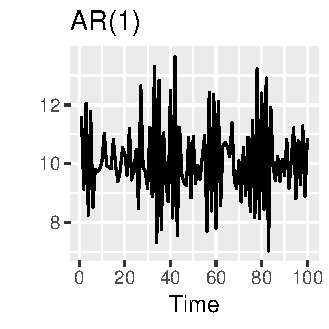
\includegraphics[width=0.5\linewidth]{week_5_arima_files/figure-beamer/unnamed-chunk-20-1}

\end{frame}

\begin{frame}{AR(1) model}

\begin{block}{}
\centerline{$y_{t}    =   c + \phi_1 y_{t - 1}  +  \varepsilon_{t}$}
\end{block}

\begin{itemize}
\tightlist
\item
  When \(\phi_1=0\), \(y_t\) is \textbf{equivalent to WN}
\item
  When \(\phi_1=1\) and \(c=0\), \(y_t\) is \textbf{equivalent to a RW}
\item
  When \(\phi_1=1\) and \(c\ne0\), \(y_t\) is \textbf{equivalent to a RW
  with drift}
\item
  When \(\phi_1<0\), \(y_t\) tends to \textbf{oscillate between positive
  and negative values}.
\end{itemize}

\end{frame}

\begin{frame}{AR(2) model}

\begin{block}{}
\centerline{$y_t = 8 + 1.3y_{t-1} - 0.7 y_{t-2} + \varepsilon_t$}
\end{block}

\rightline{$\varepsilon_t\sim N(0,1)$, \qquad $T=100$.}

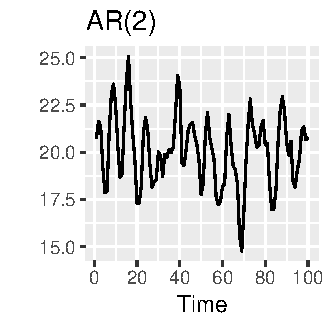
\includegraphics[width=0.5\linewidth]{week_5_arima_files/figure-beamer/unnamed-chunk-21-1}

\end{frame}

\begin{frame}{Stationarity conditions}

We normally restrict autoregressive models to stationary data, and then
some constraints on the values of the parameters are required.

\begin{block}{General condition for stationarity}
Complex roots of $1-\phi_1 z - \phi_2 z^2 - \dots - \phi_pz^p$ lie outside the unit circle on the complex plane.
\end{block}

\pause

\begin{itemize}
\tightlist
\item
  For \(p=1\): \(-1<\phi_1<1\).
\item
  For
  \(p=2\):\newline \(-1<\phi_2<1\qquad \phi_2+\phi_1 < 1 \qquad \phi_2 -\phi_1 < 1\).
\item
  More complicated conditions hold for \(p\ge3\).
\item
  Estimation software takes care of this.
\end{itemize}

\end{frame}

\begin{frame}{Moving Average (MA) models}

\begin{block}{Moving Average (MA) models:}
$$
  y_{t}  =  c +  \varepsilon_t + \theta_{1}\varepsilon_{t - 1}  +  \theta_{2}\varepsilon_{t - 2}  +  \cdots  + \theta_{q}\varepsilon_{t - q},
$$
where $\varepsilon_t$ is white noise.
This is a multiple regression with  \textbf{past \emph{errors}}
as predictors. \emph{Don't confuse this with moving average smoothing!}
\end{block}

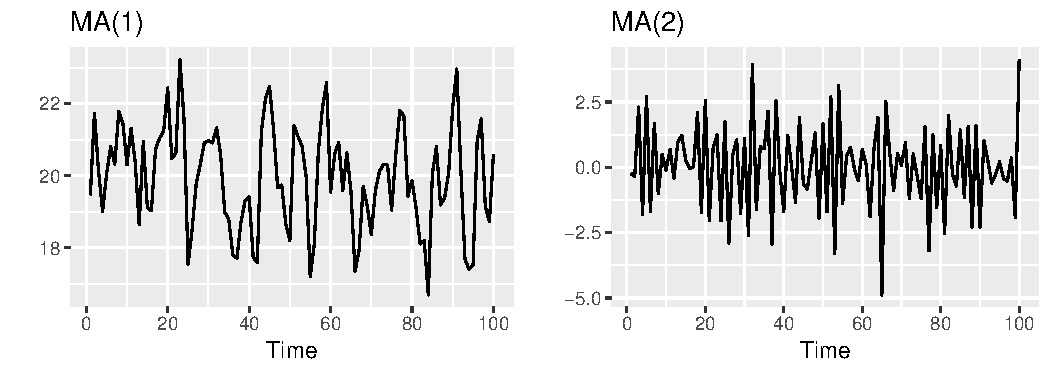
\includegraphics{week_5_arima_files/figure-beamer/maq-1.pdf}

\end{frame}

\begin{frame}{MA(1) model}

\begin{block}{}
\centerline{$y_t = 20 + \varepsilon_t + 0.8 \varepsilon_{t-1}$}
\end{block}

\rightline{$\varepsilon_t\sim N(0,1)$,\quad $T=100$.}

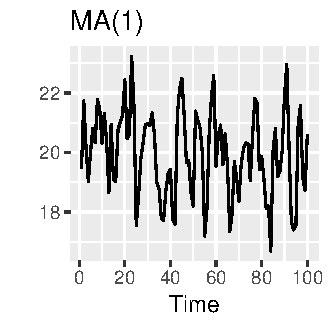
\includegraphics[width=0.5\linewidth]{week_5_arima_files/figure-beamer/unnamed-chunk-22-1}

\end{frame}

\begin{frame}{MA(2) model}

\begin{block}{}
\centerline{$y_t = \varepsilon_t -\varepsilon_{t-1} + 0.8 \varepsilon_{t-2}$}
\end{block}

\rightline{$\varepsilon_t\sim N(0,1)$,\quad $T=100$.}

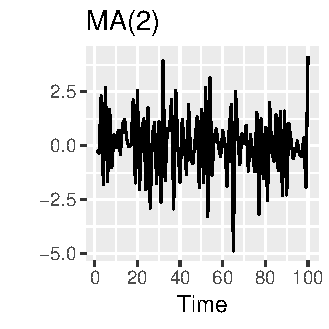
\includegraphics[width=0.5\linewidth]{week_5_arima_files/figure-beamer/unnamed-chunk-23-1}

\end{frame}

\begin{frame}{MA(\(\infty\)) models}

It is possible to write any stationary AR(\(p\)) process as an
MA(\(\infty\)) process.

\textbf{Example: AR(1)}

\begin{align*}
y_t &= \phi_1y_{t-1} + \varepsilon_t\\
&= \phi_1(\phi_1y_{t-2} + \varepsilon_{t-1}) + \varepsilon_t\\
&= \phi_1^2y_{t-2} + \phi_1 \varepsilon_{t-1} + \varepsilon_t\\
&= \phi_1^3y_{t-3} + \phi_1^2\varepsilon_{t-2} + \phi_1 \varepsilon_{t-1} + \varepsilon_t\\
&\dots
\end{align*}

\pause
Provided \(-1 < \phi_1 < 1\):
\[ y_t = \varepsilon_t + \phi_1 \varepsilon_{t-1} + \phi_1^2 \varepsilon_{t-2} + \phi_1^3 \varepsilon_{t-3} + \cdots
\]

\end{frame}

\begin{frame}{Invertibility}

\begin{itemize}
\tightlist
\item
  Any MA(\(q\)) process can be written as an AR(\(\infty\)) process if
  we impose some constraints on the MA parameters.
\item
  Then the MA model is called ``invertible''.
\item
  Invertible models have some mathematical properties that make them
  easier to use in practice.
\item
  Invertibility of an ARIMA model is equivalent to forecastability of an
  ETS model.
\end{itemize}

\end{frame}

\begin{frame}{Invertibility}

\begin{block}{General condition for invertibility}
Complex roots of $1+\theta_1 z + \theta_2 z^2 + \dots + \theta_qz^q$ lie outside the unit circle on the complex plane.
\end{block}

\pause

\begin{itemize}
\tightlist
\item
  For \(q=1\): \(-1<\theta_1<1\).
\item
  For
  \(q=2\):\newline \(-1<\theta_2<1\qquad \theta_2+\theta_1 >-1 \qquad \theta_1 -\theta_2 < 1\).
\item
  More complicated conditions hold for \(q\ge3\).
\item
  Estimation software takes care of this.
\end{itemize}

\end{frame}

\begin{frame}{ARIMA models}

\begin{block}{Autoregressive Moving Average models:}
\begin{align*}
y_{t}  &=  c  +  \phi_{1}y_{t - 1}  +  \cdots  +  \phi_{p}y_{t - p} \\
& \hspace*{2.4cm}\text{} + \theta_{1}\varepsilon_{t - 1} +  \cdots  + \theta_{q}\varepsilon_{t - q} +  \varepsilon_{t}.
\end{align*}
\end{block}

\pause

\begin{itemize}
\tightlist
\item
  Predictors include both \textbf{lagged values of \(y_t\) and lagged
  errors.}
\item
  Conditions on coefficients ensure stationarity.
\item
  Conditions on coefficients ensure invertibility. \pause
\end{itemize}

\begin{block}{Autoregressive Integrated Moving Average models}

\begin{itemize}
\tightlist
\item
  Combine ARMA model with \textbf{differencing}.
\item
  \((1-B)^d y_t\) follows an ARMA model.
\end{itemize}

\end{block}

\end{frame}

\begin{frame}{ARIMA models}

\structure{Autoregressive Integrated Moving Average models}

\begin{block}{ARIMA($p, d, q$) model}
\begin{tabular}{rl}
AR:& $p =$  order of the autoregressive part\\
I: & $d =$  degree of first differencing involved\\
MA:& $q =$  order of the moving average part.
\end{tabular}
\end{block}

\begin{itemize}
\tightlist
\item
  White noise model: ARIMA(0,0,0)
\item
  Random walk: ARIMA(0,1,0) with no constant
\item
  Random walk with drift: ARIMA(0,1,0) with \rlap{const.}
\item
  AR(\(p\)): ARIMA(\(p\),0,0)
\item
  MA(\(q\)): ARIMA(0,0,\(q\))
\end{itemize}

\end{frame}

\begin{frame}{Backshift notation for ARIMA}

\begin{itemize}
\item
  ARMA model:\vspace*{-1cm}\newline
  \parbox{12cm}{\small\begin{align*}
  \hspace*{-1cm} 
  y_{t}  &=  c + \phi_{1}By_{t} + \cdots + \phi_pB^py_{t}
         +  \varepsilon_{t}  +  \theta_{1}B\varepsilon_{t} + \cdots + \theta_qB^q\varepsilon_{t} \\
  \hspace*{-1cm} 
  \text{or}\quad & (1-\phi_1B - \cdots - \phi_p B^p) y_t = c + (1 + \theta_1 B + \cdots + \theta_q B^q)\varepsilon_t
  \end{align*}}
\item
  ARIMA(1,1,1) model:
\end{itemize}

\[
\begin{array}{c c c c}
(1 - \phi_{1} B) & (1  -  B) y_{t} &= &c + (1  + \theta_{1} B) \varepsilon_{t}\\
{\uparrow}  & {\uparrow}    &   &{\uparrow}\\
{\text{AR(1)}} & {\text{First}}   &     &{\text{MA(1)}}\\
& {\hbox to 0cm{\hss\text{difference}\hss}}\\
\end{array}
\]\pause
Written out:
\[y_t =   c + y_{t-1} + \phi_1 y_{t-1}- \phi_1 y_{t-2} + \theta_1\varepsilon_{t-1} + \varepsilon_t \]

\end{frame}

\begin{frame}{R model}

\fontsize{13}{16}\sf

\begin{block}{Intercept form}
\centerline{$(1-\phi_1B - \cdots - \phi_p B^p) y_t' = c + (1 + \theta_1 B + \cdots + \theta_q B^q)\varepsilon_t$}
\end{block}

\begin{block}{Mean form}
\centerline{$(1-\phi_1B - \cdots - \phi_p B^p)(y_t' - \mu) = (1 + \theta_1 B + \cdots + \theta_q B^q)\varepsilon_t$}
\end{block}

\begin{itemize}
\tightlist
\item
  \(y_t' = (1-B)^d y_t\)
\item
  \(\mu\) is the mean of \(y_t'\).
\item
  \(c = \mu(1-\phi_1 - \cdots - \phi_p )\).
\end{itemize}

\end{frame}

\begin{frame}{US personal consumption}

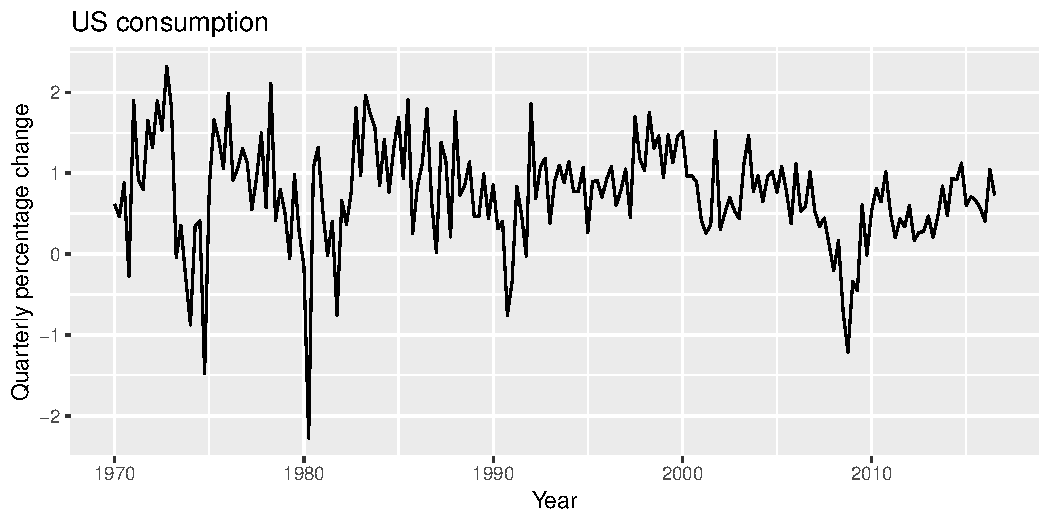
\includegraphics{week_5_arima_files/figure-beamer/unnamed-chunk-24-1.pdf}

\end{frame}

\begin{frame}[fragile]{US personal consumption}

\fontsize{10}{11}\sf

\begin{Shaded}
\begin{Highlighting}[]
\NormalTok{(fit <-}\StringTok{ }\KeywordTok{auto.arima}\NormalTok{(uschange[,}\StringTok{"Consumption"}\NormalTok{]))}
\end{Highlighting}
\end{Shaded}

\begin{verbatim}
## Series: uschange[, "Consumption"] 
## ARIMA(2,0,2) with non-zero mean 
## 
## Coefficients:
##          ar1      ar2      ma1     ma2    mean
##       1.3908  -0.5813  -1.1800  0.5584  0.7463
## s.e.  0.2553   0.2078   0.2381  0.1403  0.0845
## 
## sigma^2 estimated as 0.3511:  log likelihood=-165.14
## AIC=342.28   AICc=342.75   BIC=361.67
\end{verbatim}

\pause\vfill

```

\begin{block}{ARIMA(2,0,2) model:}

\centerline{$
  y_t = c + 1.391y_{t-1}
          -0.581 y_{t-2}
          -1.180 \varepsilon_{t-1}
          + 0.558 \varepsilon_{t-2}
          + \varepsilon_{t},
$}

where \(c= 0.746 \times (1 - 1.391 + 0.581) = 0.142\) and
\(\varepsilon_t\) is white noise with a standard deviation of
\(0.593 = \sqrt{0.351}\).

\end{block}

\end{frame}

\begin{frame}[fragile]{US personal consumption}

\fontsize{12}{15}\sf

\begin{Shaded}
\begin{Highlighting}[]
\NormalTok{fit }\OperatorTok\StringTok{ }\KeywordTok{forecast}\NormalTok{(}\DataTypeTok{h=}\DecValTok{10}\NormalTok{) }\OperatorTok\StringTok{ }\KeywordTok{autoplot}\NormalTok{(}\DataTypeTok{include=}\DecValTok{80}\NormalTok{)}
\end{Highlighting}
\end{Shaded}

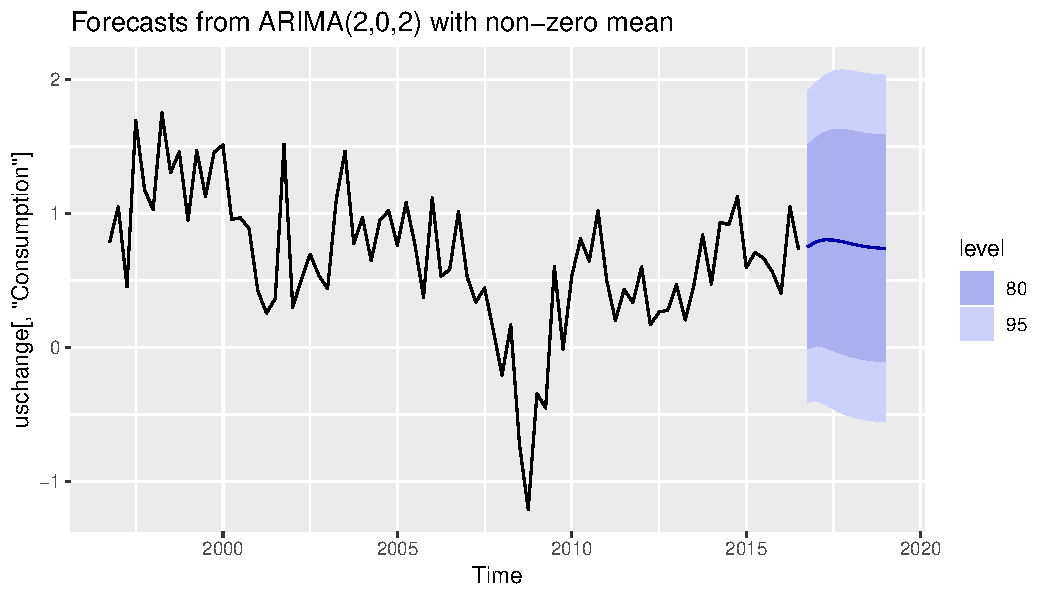
\includegraphics{week_5_arima_files/figure-beamer/unnamed-chunk-27-1.pdf}

\end{frame}

\begin{frame}{Understanding ARIMA models}

\fontsize{14}{16}\sf

\begin{itemize}
\item
  If \(c=0\) and \(d=0\), the long-term forecasts will go to zero.
\item
  If \(c=0\) and \(d=1\), the long-term forecasts will go to a non-zero
  constant.
\item
  If \(c=0\) and \(d=2\), the long-term forecasts will follow a straight
  line.
\item
  If \(c\ne0\) and \(d=0\), the long-term forecasts will go to the mean
  of the data.
\item
  If \(c\ne0\) and \(d=1\), the long-term forecasts will follow a
  straight line.
\item
  If \(c\ne0\) and \(d=2\), the long-term forecasts will follow a
  quadratic trend.
\end{itemize}

\end{frame}

\begin{frame}{Understanding ARIMA models}

\fontsize{14}{15.5}\sf

\begin{block}{Forecast variance and \(d\)}

\begin{itemize}
\tightlist
\item
  The higher the value of \(d\), the more rapidly the prediction
  intervals increase in size.
\item
  For \(d=0\), the long-term forecast standard deviation will go to the
  standard deviation of the historical data.
\end{itemize}

\end{block}

\begin{block}{Cyclic behaviour}

\begin{itemize}
\tightlist
\item
  For cyclic forecasts, \(p\ge2\) and some restrictions on coefficients
  are required.
\item
  If \(p=2\), we need \(\phi_1^2+4\phi_2<0\). Then average cycle of
  length \[
    (2\pi)/\left[\text{arc cos}(-\phi_1(1-\phi_2)/(4\phi_2))\right].
  \]
\end{itemize}

\end{block}

\end{frame}

\section{Estimation and order
selection}\label{estimation-and-order-selection}

\begin{frame}[fragile]{Maximum likelihood estimation}

Having identified the model order, we need to estimate the parameters
\(c\), \(\phi_1,\dots,\phi_p\), \(\theta_1,\dots,\theta_q\).\pause

\begin{itemize}
\tightlist
\item
  MLE is very similar to least squares estimation obtained by minimizing
  \[\sum_{t-1}^T e_t^2.\]
\item
  The \texttt{Arima()} command allows CLS or MLE estimation.
\item
  Non-linear optimization must be used in either case.
\item
  Different software will give different estimates.
\end{itemize}

\end{frame}

\begin{frame}{Partial autocorrelations}

\structure{Partial autocorrelations} measure relationship\newline
between \(y_{t}\) and \(y_{t - k}\), when the effects of other time lags
--- \(1, 2, 3, \dots, k - 1\) --- are removed.\pause

\begin{block}{}
\begin{align*}
\alpha_k&= \text{$k$th partial autocorrelation coefficient}\\
&= \text{equal to the estimate of $b_k$ in regression:}\\
& \hspace*{0.8cm} y_t = c + \phi_1 y_{t-1} + \phi_2 y_{t-2} + \dots + \phi_k y_{t-k}.
\end{align*}
\end{block}

\pause

\begin{itemize}
\tightlist
\item
  Varying number of terms on RHS gives \(\alpha_k\) for different values
  of \(k\).
\item
  There are more efficient ways of calculating \(\alpha_k\).
\item
  \(\alpha_1=\rho_1\)
\item
  same critical values of \(\pm 1.96/\sqrt{T}\) as for ACF.
\end{itemize}

\end{frame}

\begin{frame}{Example: US consumption}

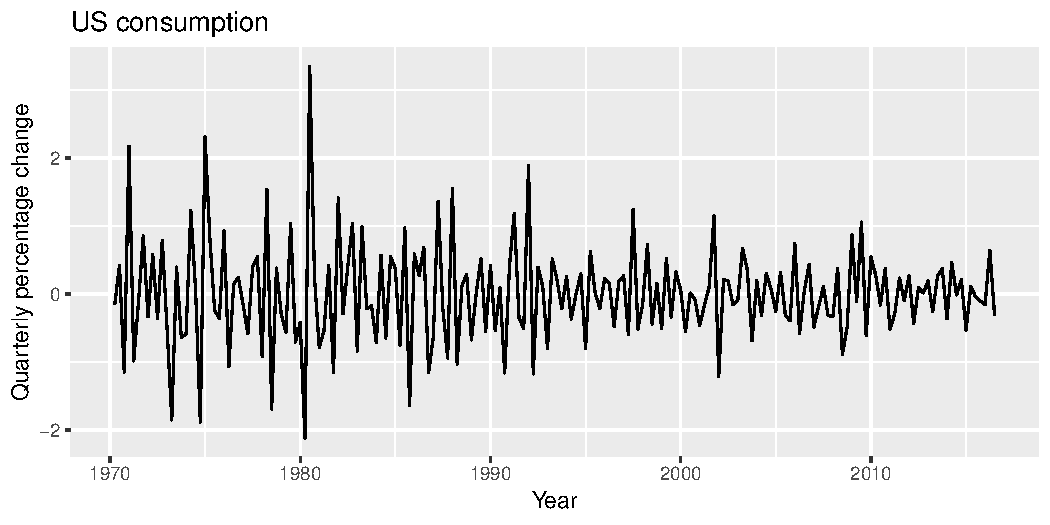
\includegraphics{week_5_arima_files/figure-beamer/unnamed-chunk-28-1.pdf}

\end{frame}

\begin{frame}{Example: US consumption}

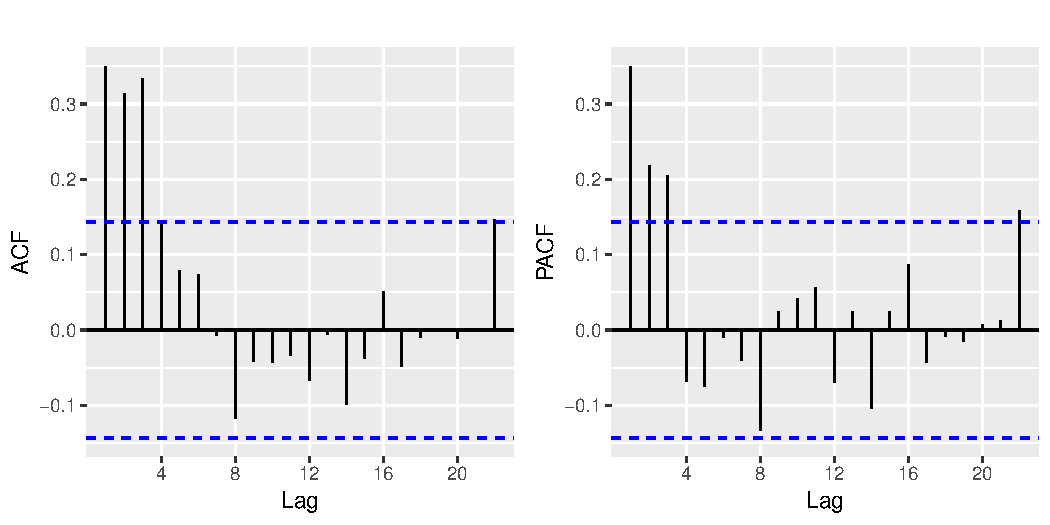
\includegraphics{week_5_arima_files/figure-beamer/usconsumptionacf-1.pdf}

\end{frame}

\begin{frame}{ACF and PACF interpretation}

\textbf{AR(1)}

\begin{align*}
\hspace*{1cm}\rho_k &= \phi_1^k\qquad\text{for $k=1,2,\dots$};\\
\alpha_1 &= \phi_1 \qquad\alpha_k = 0\qquad\text{for $k=2,3,\dots$}.
\end{align*}

So we have an AR(1) model when

\begin{itemize}
\tightlist
\item
  autocorrelations exponentially decay
\item
  there is a single significant partial autocorrelation.
\end{itemize}

\end{frame}

\begin{frame}{ACF and PACF interpretation}

\textbf{AR(\(p\))}

\begin{itemize}
\tightlist
\item
  ACF dies out in an exponential or damped sine-wave manner
\item
  PACF has all zero spikes beyond the \(p\)th spike
\end{itemize}

So we have an AR(\(p\)) model when

\begin{itemize}
\tightlist
\item
  the ACF is exponentially decaying or sinusoidal
\item
  there is a significant spike at lag \(p\) in PACF, but none beyond
  \(p\)
\end{itemize}

\end{frame}

\begin{frame}{ACF and PACF interpretation}

\textbf{MA(1)}

\begin{align*}
\hspace*{1cm}\rho_1 &= \theta_1\qquad \rho_k = 0\qquad\text{for $k=2,3,\dots$};\\
\alpha_k &= -(-\theta_1)^k
\end{align*}

So we have an MA(1) model when

\begin{itemize}
\tightlist
\item
  the PACF is exponentially decaying and
\item
  there is a single significant spike in ACF
\end{itemize}

\end{frame}

\begin{frame}{ACF and PACF interpretation}

\textbf{MA(\(q\))}

\begin{itemize}
\tightlist
\item
  PACF dies out in an exponential or damped sine-wave manner
\item
  ACF has all zero spikes beyond the \(q\)th spike
\end{itemize}

So we have an MA(\(q\)) model when

\begin{itemize}
\tightlist
\item
  the PACF is exponentially decaying or sinusoidal
\item
  there is a significant spike at lag \(q\) in ACF, but none beyond
  \(q\)
\end{itemize}

\end{frame}

\begin{frame}{Example: Mink trapping}

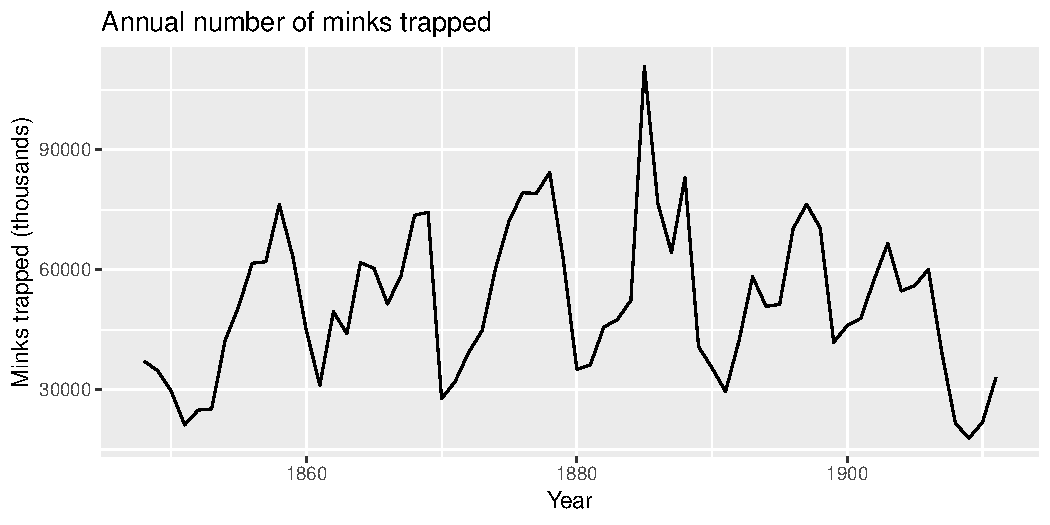
\includegraphics{week_5_arima_files/figure-beamer/unnamed-chunk-29-1.pdf}

\end{frame}

\begin{frame}{Example: Mink trapping}

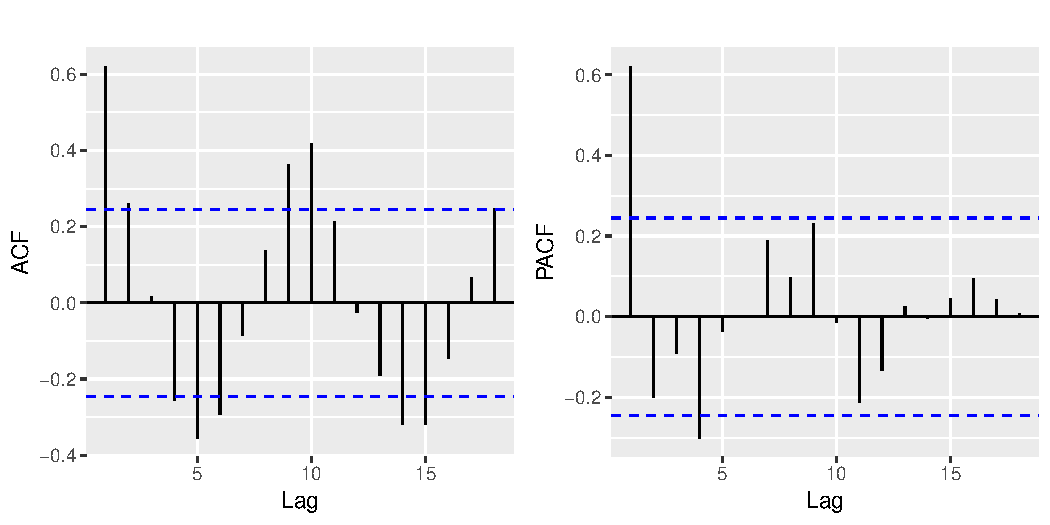
\includegraphics{week_5_arima_files/figure-beamer/unnamed-chunk-30-1.pdf}

\end{frame}

\begin{frame}{Information criteria}

\structure{Akaike's Information Criterion (AIC):}
\centerline{$\text{AIC} = -2 \log(L) + 2(p+q+k+1),$} where \(L\) is the
likelihood of the data,\newline
\(k=1\) if \(c\ne0\) and \(k=0\) if \(c=0\).\pause\vspace*{0.2cm}

\structure{Corrected AIC:}
\centerline{$\text{AICc} = \text{AIC} + \frac{2(p+q+k+1)(p+q+k+2)}{T-p-q-k-2}.$}\pause\vspace*{0.2cm}

\structure{Bayesian Information Criterion:}
\centerline{$\text{BIC} = \text{AIC} + [\log(T)-2](p+q+k-1).$}
\pause\vspace*{-0.2cm}

\begin{block}{}Good models are obtained by minimizing either the AIC, \text{AICc}\ or BIC\@. Our preference is to use the \text{AICc}.\end{block}

\end{frame}

\section{ARIMA modelling in R}\label{arima-modelling-in-r}

\begin{frame}{How does auto.arima() work?}

\begin{block}{A non-seasonal ARIMA process}
\[
\phi(B)(1-B)^dy_{t} = c + \theta(B)\varepsilon_t
\]
Need to select appropriate orders: \alert{$p,q, d$}
\end{block}

\structure{Hyndman and Khandakar (JSS, 2008) algorithm:}

\begin{itemize}
\tightlist
\item
  Select no.~differences \alert{$d$} and \alert{$D$} via KPSS test and
  seasonal strength measure.
\item
  Select \alert{$p,q$} by minimising AICc.
\item
  Use stepwise search to traverse model space.
\end{itemize}

\end{frame}

\begin{frame}{How does auto.arima() work?}

\fontsize{12}{13}\sf

\begin{block}{}
\centerline{$\text{AICc} = -2 \log(L) + 2(p+q+k+1)\left[1 +
\frac{(p+q+k+2)}{T-p-q-k-2}\right].$}
where $L$ is the maximised likelihood fitted to the \textit{differenced} data,
$k=1$ if $c\neq 0$ and $k=0$ otherwise.
\end{block}

\pause

\begin{description}
\item[Step1:]
Select current model (with smallest AICc) from:\newline
ARIMA\((2,d,2)\)\newline
ARIMA\((0,d,0)\)\newline
ARIMA\((1,d,0)\)\newline
ARIMA\((0,d,1)\) \pause\vspace*{-0.1cm}
\item[Step 2:]
Consider variations of current model:

\begin{itemize}
\tightlist
\item
  vary one of \(p,q,\) from current model by \(\pm1\);
\item
  \(p,q\) both vary from current model by \(\pm1\);
\item
  Include/exclude \(c\) from current model.
\end{itemize}
\end{description}

Model with lowest AICc becomes current model.

\structure{Repeat Step 2 until no lower AICc can be found.}

\end{frame}

\begin{frame}[fragile]{Choosing your own model}

\begin{Shaded}
\begin{Highlighting}[]
\KeywordTok{ggtsdisplay}\NormalTok{(internet)}
\end{Highlighting}
\end{Shaded}

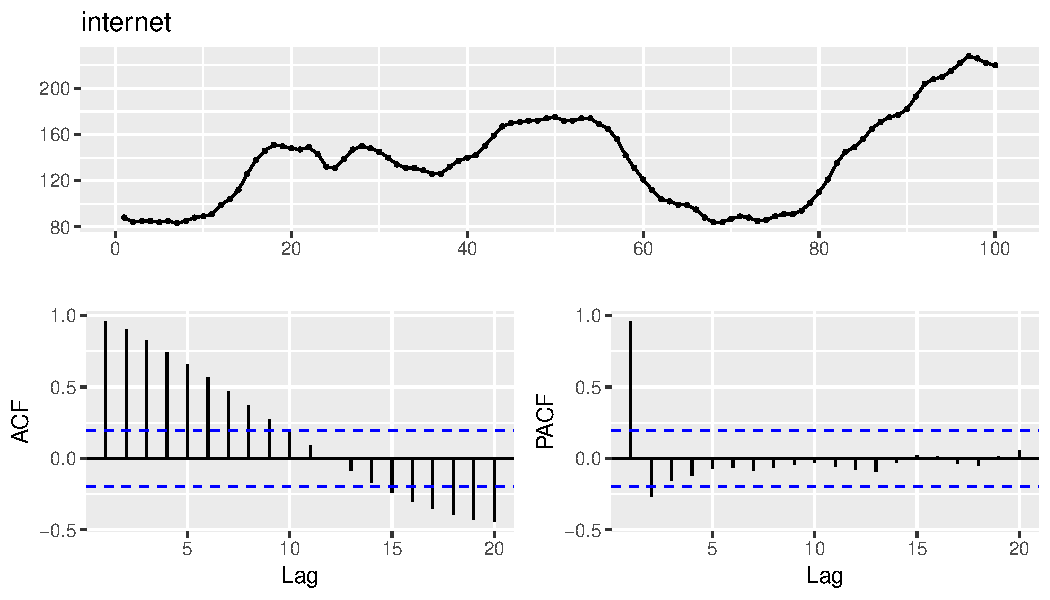
\includegraphics{week_5_arima_files/figure-beamer/unnamed-chunk-31-1.pdf}

\end{frame}

\begin{frame}[fragile]{Choosing your own model}

\begin{Shaded}
\begin{Highlighting}[]
\KeywordTok{ggtsdisplay}\NormalTok{(}\KeywordTok{diff}\NormalTok{(internet))}
\end{Highlighting}
\end{Shaded}

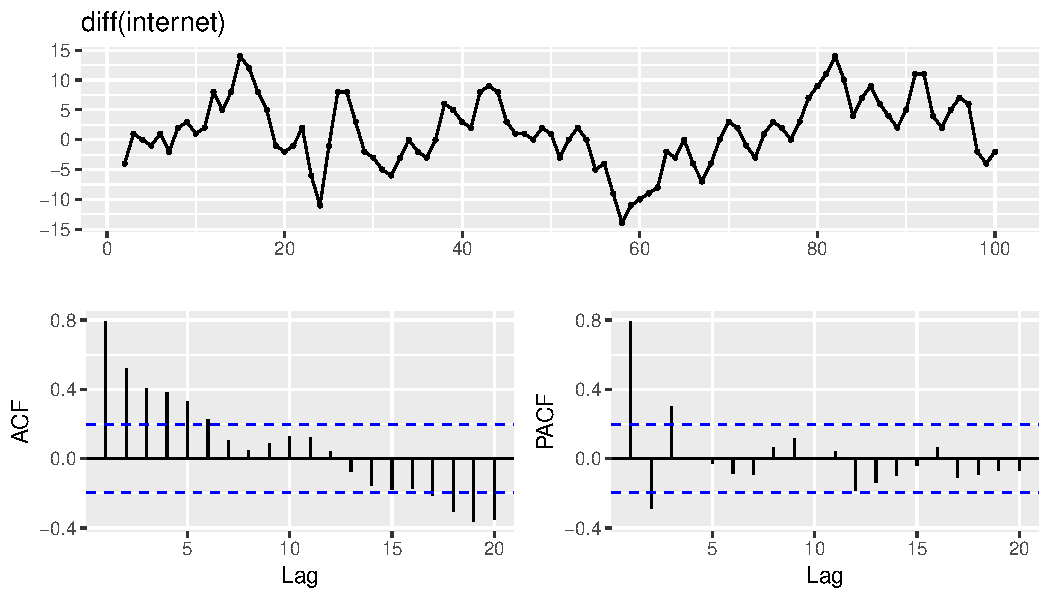
\includegraphics{week_5_arima_files/figure-beamer/unnamed-chunk-32-1.pdf}

\end{frame}

\begin{frame}[fragile]{Choosing your own model}

\fontsize{13}{14}\sf

\begin{Shaded}
\begin{Highlighting}[]
\NormalTok{(fit <-}\StringTok{ }\KeywordTok{Arima}\NormalTok{(internet,}\DataTypeTok{order=}\KeywordTok{c}\NormalTok{(}\DecValTok{3}\NormalTok{,}\DecValTok{1}\NormalTok{,}\DecValTok{0}\NormalTok{)))}
\end{Highlighting}
\end{Shaded}

\begin{verbatim}
## Series: internet 
## ARIMA(3,1,0) 
## 
## Coefficients:
##          ar1      ar2     ar3
##       1.1513  -0.6612  0.3407
## s.e.  0.0950   0.1353  0.0941
## 
## sigma^2 estimated as 9.656:  log likelihood=-252
## AIC=511.99   AICc=512.42   BIC=522.37
\end{verbatim}

\end{frame}

\begin{frame}[fragile]{Choosing your own model}

\fontsize{13}{14}\sf

\begin{Shaded}
\begin{Highlighting}[]
\KeywordTok{auto.arima}\NormalTok{(internet)}
\end{Highlighting}
\end{Shaded}

\begin{verbatim}
## Series: internet 
## ARIMA(1,1,1) 
## 
## Coefficients:
##          ar1     ma1
##       0.6504  0.5256
## s.e.  0.0842  0.0896
## 
## sigma^2 estimated as 9.995:  log likelihood=-254.15
## AIC=514.3   AICc=514.55   BIC=522.08
\end{verbatim}

\end{frame}

\begin{frame}[fragile]{Choosing your own model}

\fontsize{13}{14}\sf

\begin{Shaded}
\begin{Highlighting}[]
\KeywordTok{auto.arima}\NormalTok{(internet, }\DataTypeTok{stepwise=}\OtherTok{FALSE}\NormalTok{,}
  \DataTypeTok{approximation=}\OtherTok{FALSE}\NormalTok{)}
\end{Highlighting}
\end{Shaded}

\begin{verbatim}
## Series: internet 
## ARIMA(3,1,0) 
## 
## Coefficients:
##          ar1      ar2     ar3
##       1.1513  -0.6612  0.3407
## s.e.  0.0950   0.1353  0.0941
## 
## sigma^2 estimated as 9.656:  log likelihood=-252
## AIC=511.99   AICc=512.42   BIC=522.37
\end{verbatim}

\end{frame}

\begin{frame}[fragile]{Choosing your own model}

\begin{Shaded}
\begin{Highlighting}[]
\KeywordTok{checkresiduals}\NormalTok{(fit)}
\end{Highlighting}
\end{Shaded}

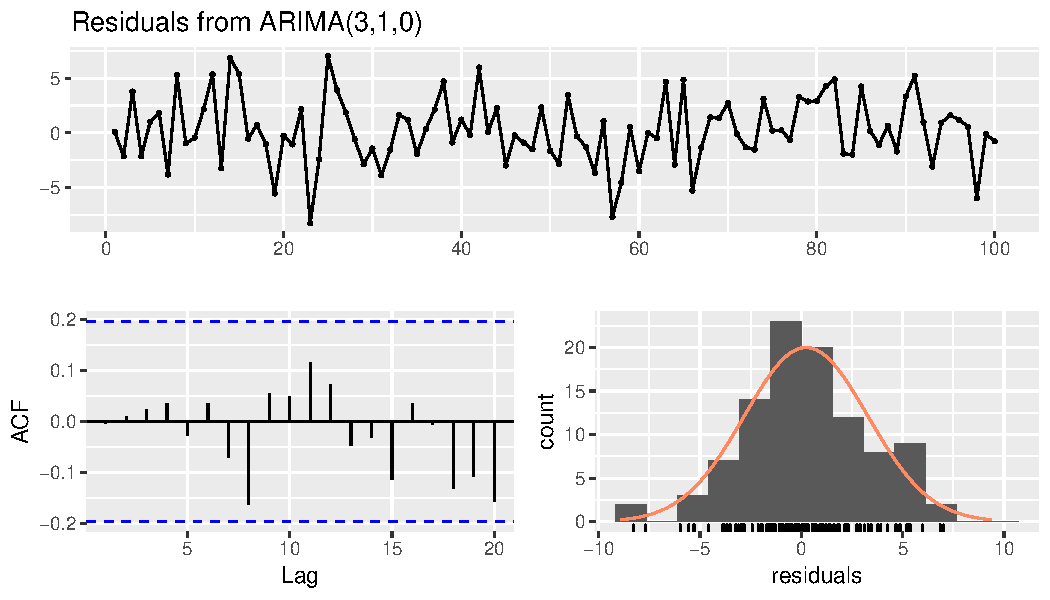
\includegraphics{week_5_arima_files/figure-beamer/unnamed-chunk-35-1.pdf}

\end{frame}

\begin{frame}[fragile]{Choosing your own model}

\begin{verbatim}
## 
##  Ljung-Box test
## 
## data:  Residuals from ARIMA(3,1,0)
## Q* = 4.4913, df = 7, p-value = 0.7218
## 
## Model df: 3.   Total lags used: 10
\end{verbatim}

\end{frame}

\begin{frame}[fragile]{Choosing your own model}

\begin{Shaded}
\begin{Highlighting}[]
\NormalTok{fit }\OperatorTok\StringTok{ }\NormalTok{forecast }\OperatorTok\StringTok{ }\NormalTok{autoplot}
\end{Highlighting}
\end{Shaded}

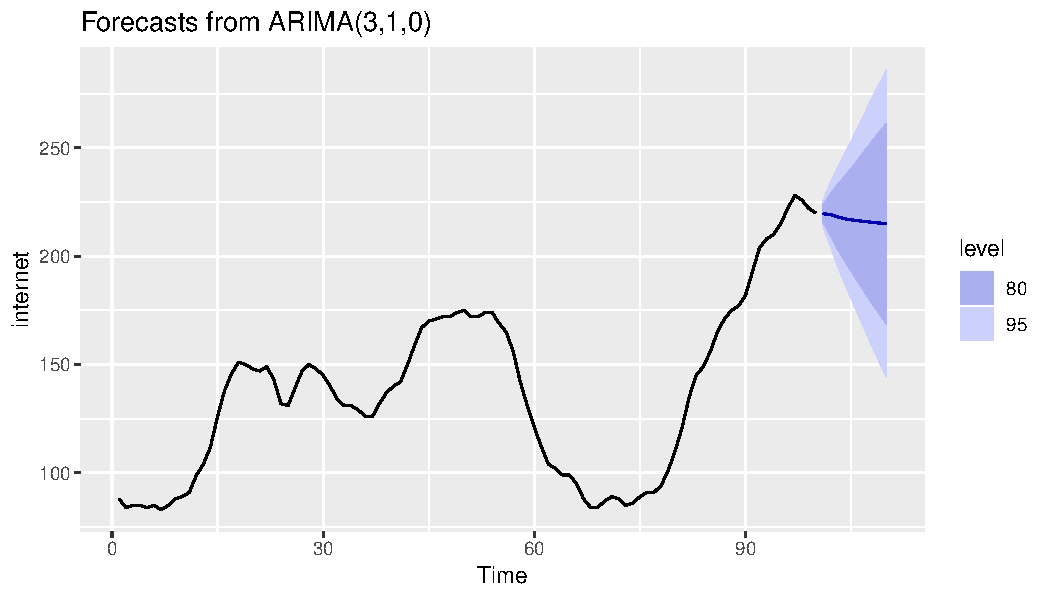
\includegraphics{week_5_arima_files/figure-beamer/unnamed-chunk-37-1.pdf}

\end{frame}

\begin{frame}{Modelling procedure with \texttt{Arima}}

\fontsize{12}{13}\sf

\begin{enumerate}
\def\labelenumi{\arabic{enumi}.}
\tightlist
\item
  Plot the data. Identify any unusual observations.
\item
  If necessary, transform the data (using a Box-Cox transformation) to
  stabilize the variance.
\item
  If the data are non-stationary: take first differences of the data
  until the data are stationary.
\item
  Examine the ACF/PACF: Is an AR(\(p\)) or MA(\(q\)) model appropriate?
\item
  Try your chosen model(s), and use the \text{AICc} to search for a
  better model.
\item
  Check the residuals from your chosen model by plotting the ACF of the
  residuals, and doing a portmanteau test of the residuals. If they do
  not look like white noise, try a modified model.
\item
  Once the residuals look like white noise, calculate forecasts.
\end{enumerate}

\end{frame}

\begin{frame}[fragile]{Modelling procedure with \texttt{auto.arima}}

\fontsize{12}{13}\sf

\begin{enumerate}
\def\labelenumi{\arabic{enumi}.}
\tightlist
\item
  Plot the data. Identify any unusual observations.
\item
  If necessary, transform the data (using a Box-Cox transformation) to
  stabilize the variance.
\end{enumerate}

\vspace*{1.15cm}

\begin{enumerate}
\def\labelenumi{\arabic{enumi}.}
\setcounter{enumi}{2}
\tightlist
\item
  Use \texttt{auto.arima} to select a model.
\end{enumerate}

\vspace*{1.15cm}

\begin{enumerate}
\def\labelenumi{\arabic{enumi}.}
\setcounter{enumi}{5}
\tightlist
\item
  Check the residuals from your chosen model by plotting the ACF of the
  residuals, and doing a portmanteau test of the residuals. If they do
  not look like white noise, try a modified model.
\item
  Once the residuals look like white noise, calculate forecasts.
\end{enumerate}

\end{frame}

\begin{frame}{Modelling procedure}

\centerline{\includegraphics[height=8.cm]{Figure-8-10}}

\end{frame}

\begin{frame}[fragile]{\large Seasonally adjusted electrical equipment}

\fontsize{11.5}{15}\sf

\begin{Shaded}
\begin{Highlighting}[]
\NormalTok{eeadj <-}\StringTok{ }\KeywordTok{seasadj}\NormalTok{(}\KeywordTok{stl}\NormalTok{(elecequip, }\DataTypeTok{s.window=}\StringTok{"periodic"}\NormalTok{))}
\KeywordTok{autoplot}\NormalTok{(eeadj) }\OperatorTok{+}\StringTok{ }\KeywordTok{xlab}\NormalTok{(}\StringTok{"Year"}\NormalTok{) }\OperatorTok{+}
\StringTok{  }\KeywordTok{ylab}\NormalTok{(}\StringTok{"Seasonally adjusted new orders index"}\NormalTok{)}
\end{Highlighting}
\end{Shaded}

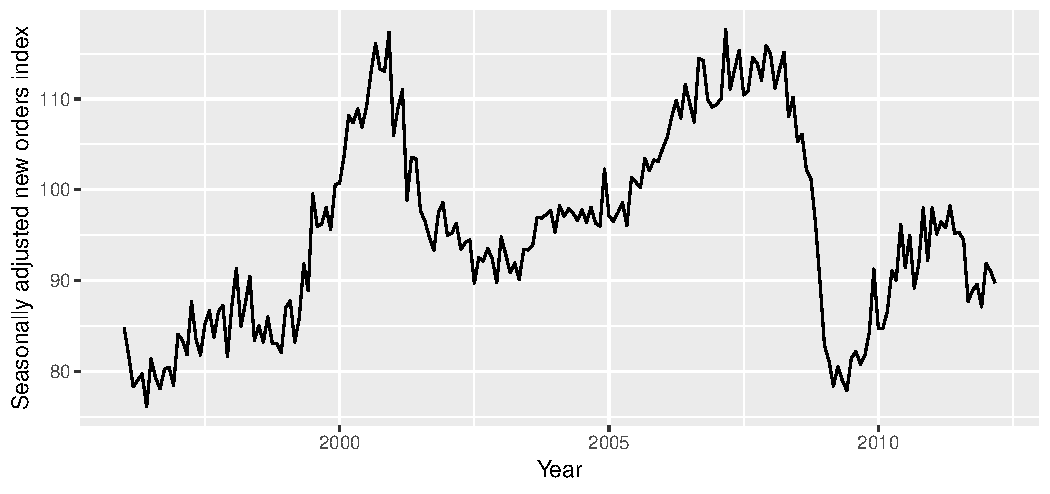
\includegraphics{week_5_arima_files/figure-beamer/ee1-1.pdf}

\end{frame}

\begin{frame}{\large Seasonally adjusted electrical equipment}

\begin{enumerate}
\def\labelenumi{\arabic{enumi}.}
\tightlist
\item
  Time plot shows sudden changes, particularly big drop in 2008/2009 due
  to global economic environment. Otherwise nothing unusual and no need
  for data adjustments.
\item
  No evidence of changing variance, so no Box-Cox transformation.
\item
  Data are clearly non-stationary, so we take first differences.
\end{enumerate}

\end{frame}

\begin{frame}[fragile]{\large Seasonally adjusted electrical equipment}

\begin{Shaded}
\begin{Highlighting}[]
\KeywordTok{ggtsdisplay}\NormalTok{(}\KeywordTok{diff}\NormalTok{(eeadj))}
\end{Highlighting}
\end{Shaded}

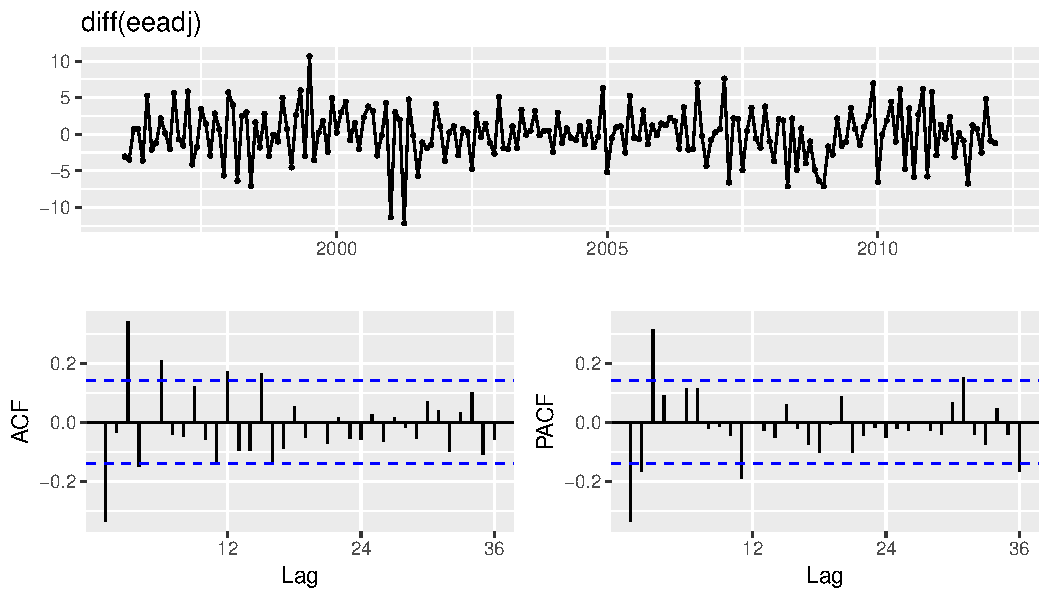
\includegraphics{week_5_arima_files/figure-beamer/ee2-1.pdf}

\end{frame}

\begin{frame}{\large Seasonally adjusted electrical equipment}

\begin{enumerate}
\def\labelenumi{\arabic{enumi}.}
\setcounter{enumi}{3}
\tightlist
\item
  PACF is suggestive of AR(3). So initial candidate model is
  ARIMA(3,1,0). No other obvious candidates.
\item
  Fit ARIMA(3,1,0) model along with variations: ARIMA(4,1,0),
  ARIMA(2,1,0), ARIMA(3,1,1), etc. ARIMA(3,1,1) has smallest \text{AICc}
  value.
\end{enumerate}

\end{frame}

\begin{frame}[fragile]{\large Seasonally adjusted electrical equipment}

\fontsize{10}{10}\sf

\begin{Shaded}
\begin{Highlighting}[]
\NormalTok{(fit <-}\StringTok{ }\KeywordTok{Arima}\NormalTok{(eeadj, }\DataTypeTok{order=}\KeywordTok{c}\NormalTok{(}\DecValTok{3}\NormalTok{,}\DecValTok{1}\NormalTok{,}\DecValTok{1}\NormalTok{)))}
\end{Highlighting}
\end{Shaded}

\begin{verbatim}
## Series: eeadj 
## ARIMA(3,1,1) 
## 
## Coefficients:
##          ar1     ar2     ar3      ma1
##       0.0044  0.0916  0.3698  -0.3921
## s.e.  0.2201  0.0984  0.0669   0.2426
## 
## sigma^2 estimated as 9.577:  log likelihood=-492.69
## AIC=995.38   AICc=995.7   BIC=1011.72
\end{verbatim}

\end{frame}

\begin{frame}[fragile]{\large Seasonally adjusted electrical equipment}

\begin{enumerate}
\def\labelenumi{\arabic{enumi}.}
\setcounter{enumi}{5}
\tightlist
\item
  ACF plot of residuals from ARIMA(3,1,1) model look like white noise.
\end{enumerate}

\fontsize{11}{11}\sf

\begin{Shaded}
\begin{Highlighting}[]
\KeywordTok{checkresiduals}\NormalTok{(fit)}
\end{Highlighting}
\end{Shaded}

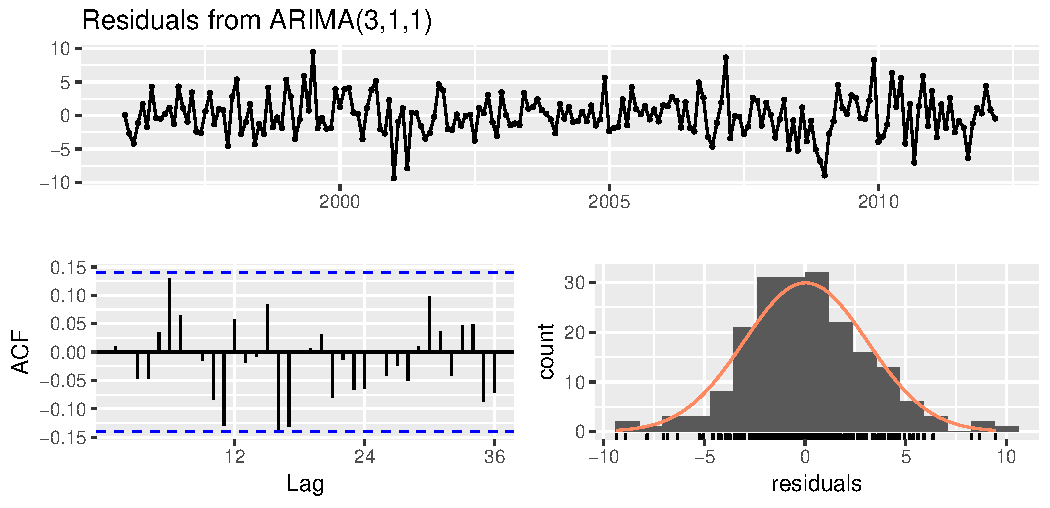
\includegraphics{week_5_arima_files/figure-beamer/unnamed-chunk-39-1.pdf}

\begin{verbatim}
## 
##  Ljung-Box test
## 
## data:  Residuals from ARIMA(3,1,1)
## Q* = 24.034, df = 20, p-value = 0.2409
## 
## Model df: 4.   Total lags used: 24
\end{verbatim}

\end{frame}

\begin{frame}[fragile]{\large Seasonally adjusted electrical equipment}

\begin{verbatim}
## 
##  Ljung-Box test
## 
## data:  Residuals from ARIMA(3,1,1)
## Q* = 24.034, df = 20, p-value = 0.2409
## 
## Model df: 4.   Total lags used: 24
\end{verbatim}

\end{frame}

\begin{frame}[fragile]{\large Seasonally adjusted electrical equipment}

\begin{Shaded}
\begin{Highlighting}[]
\NormalTok{fit }\OperatorTok\StringTok{ }\NormalTok{forecast }\OperatorTok\StringTok{ }\NormalTok{autoplot}
\end{Highlighting}
\end{Shaded}

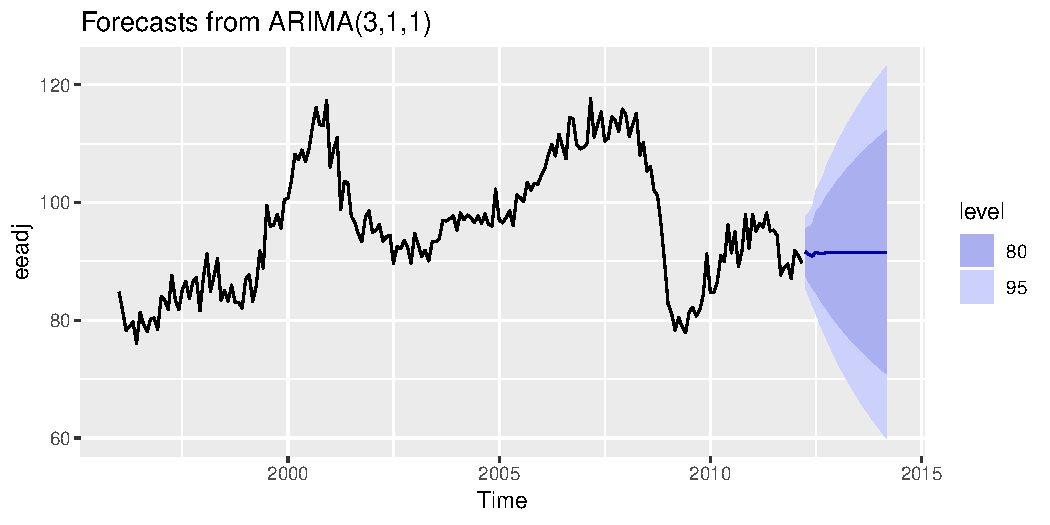
\includegraphics{week_5_arima_files/figure-beamer/unnamed-chunk-41-1.pdf}

\end{frame}

\section{Forecasting}\label{forecasting}

\begin{frame}{Point forecasts}

\begin{enumerate}
\def\labelenumi{\arabic{enumi}.}
\tightlist
\item
  Rearrange ARIMA equation so \(y_t\) is on LHS.
\item
  Rewrite equation by replacing \(t\) by \(T+h\).
\item
  On RHS, replace future observations by their forecasts, future errors
  by zero, and past errors by corresponding residuals.
\end{enumerate}

Start with \(h=1\). Repeat for \(h=2,3,\dots\).

\end{frame}

\begin{frame}{Point forecasts}

\fontsize{14}{14}\sf

\structure{ARIMA(3,1,1) forecasts: Step 1}

\begin{block}{}
\centerline{$(1-\phi_1B -\phi_2B^2-\phi_3B^3)(1-B) y_t = (1+\theta_1B)\varepsilon_{t},$}
\end{block}

\pause\vspace*{-0.4cm}

\begin{align*}
\left[1-(1+\phi_1)B +(\phi_1-\phi_2)B^2 + (\phi_2-\phi_3)B^3 +\phi_3B^4\right] y_t\\ = (1+\theta_1B)\varepsilon_{t},
\end{align*}

\pause\vspace*{-0.4cm}

\begin{align*}
y_t - (1+\phi_1)y_{t-1} +(\phi_1-\phi_2)y_{t-2} + (\phi_2-\phi_3)y_{t-3}\\ \mbox{}+\phi_3y_{t-4} = \varepsilon_t+\theta_1\varepsilon_{t-1}.
\end{align*}

\pause\vspace*{-0.4cm}

\begin{align*}
y_t = (1+\phi_1)y_{t-1} -(\phi_1-\phi_2)y_{t-2} - (\phi_2-\phi_3)y_{t-3}\\\mbox{} -\phi_3y_{t-4} + \varepsilon_t+\theta_1\varepsilon_{t-1}.
\end{align*}

\end{frame}

\begin{frame}{Point forecasts (h=1)}

\fontsize{14}{14}\sf

\begin{block}{}
\begin{align*}
y_t = (1+\phi_1)y_{t-1} -(\phi_1-\phi_2)y_{t-2} - (\phi_2-\phi_3)y_{t-3}\\\mbox{} -\phi_3y_{t-4} + \varepsilon_t+\theta_1\varepsilon_{t-1}.
\end{align*}
\end{block}

\pause
\structure{ARIMA(3,1,1) forecasts: Step 2}

\begin{align*}
y_{T+1} = (1+\phi_1)y_{T} -(\phi_1-\phi_2)y_{T-1} - (\phi_2-\phi_3)y_{T-2}\\\mbox{} -\phi_3y_{T-3} + \varepsilon_{T+1}+\theta_1\varepsilon_{T}.
\end{align*}

\pause
\structure{ARIMA(3,1,1) forecasts: Step 3}

\begin{align*}
\hat{y}_{T+1|T} = (1+\phi_1)y_{T} -(\phi_1-\phi_2)y_{T-1} - (\phi_2-\phi_3)y_{T-2}\\\mbox{} -\phi_3y_{T-3} + \theta_1 e_{T}.
\end{align*}

\end{frame}

\begin{frame}{Point forecasts (h=2)}

\fontsize{14}{14}\sf

\begin{block}{}
\begin{align*}
y_t = (1+\phi_1)y_{t-1} -(\phi_1-\phi_2)y_{t-2} - (\phi_2-\phi_3)y_{t-3}\\\mbox{} -\phi_3y_{t-4} + \varepsilon_t+\theta_1\varepsilon_{t-1}.
\end{align*}
\end{block}

\pause
\structure{ARIMA(3,1,1) forecasts: Step 2}

\begin{align*}
y_{T+2} = (1+\phi_1)y_{T+1} -(\phi_1-\phi_2)y_{T} - (\phi_2-\phi_3)y_{T-1}\\\mbox{} -\phi_3y_{T-2} + \varepsilon_{T+2}+\theta_1\varepsilon_{T+1}.
\end{align*}

\pause
\structure{ARIMA(3,1,1) forecasts: Step 3}

\begin{align*}
\hat{y}_{T+2|T} = (1+\phi_1)\hat{y}_{T+1|T} -(\phi_1-\phi_2)y_{T} - (\phi_2-\phi_3)y_{T-1}\\\mbox{} -\phi_3y_{T-2}.
\end{align*}

\end{frame}

\begin{frame}{Prediction intervals}

\begin{block}{95\% prediction interval}
$$\hat{y}_{T+h|T} \pm 1.96\sqrt{v_{T+h|T}}$$
where $v_{T+h|T}$ is estimated forecast variance.
\end{block}

\pause

\begin{itemize}
\tightlist
\item
  \(v_{T+1|T}=\hat{\sigma}^2\) for all ARIMA models regardless of
  parameters and orders.
\item
  Multi-step prediction intervals for ARIMA(0,0,\(q\)):
  \centerline{$\displaystyle y_t = \varepsilon_t + \sum_{i=1}^q \theta_i \varepsilon_{t-i}.$}
  \centerline{$\displaystyle
  v_{T|T+h} = \hat{\sigma}^2 \left[ 1 + \sum_{i=1}^{h-1} \theta_i^2\right], \qquad\text{for~} h=2,3,\dots.$}
\end{itemize}

\end{frame}

\begin{frame}{Prediction intervals}

\begin{block}{95\% Prediction interval}
$$\hat{y}_{T+h|T} \pm 1.96\sqrt{v_{T+h|T}}$$
where $v_{T+h|T}$ is estimated forecast variance.
\end{block}

\begin{itemize}
\tightlist
\item
  Multi-step prediction intervals for ARIMA(0,0,\(q\)):
  \centerline{$\displaystyle y_t = \varepsilon_t + \sum_{i=1}^q \theta_i \varepsilon_{t-i}.$}
  \centerline{$\displaystyle
  v_{T|T+h} = \hat{\sigma}^2 \left[ 1 + \sum_{i=1}^{h-1} \theta_i^2\right], \qquad\text{for~} h=2,3,\dots.$}
\end{itemize}

\pause

\begin{itemize}
\tightlist
\item
  AR(1): Rewrite as MA(\(\infty\)) and use above result.
\item
  Other models beyond scope of this subject.
\end{itemize}

\end{frame}

\begin{frame}{Prediction intervals}

\begin{itemize}
\tightlist
\item
  Prediction intervals \textbf{increase in size with forecast horizon}.
\item
  Prediction intervals can be difficult to calculate by hand
\item
  Calculations assume residuals are \textbf{uncorrelated} and
  \textbf{normally distributed}.
\item
  Prediction intervals tend to be too narrow.

  \begin{itemize}
  \tightlist
  \item
    the uncertainty in the parameter estimates has not been accounted
    for.
  \item
    the ARIMA model assumes historical patterns will not change during
    the forecast period.
  \item
    the ARIMA model assumes uncorrelated future \rlap{errors}
  \end{itemize}
\end{itemize}

\end{frame}

\begin{frame}[fragile]{Your turn}

For the \texttt{usgdp} data:

\begin{itemize}
\tightlist
\item
  if necessary, find a suitable Box-Cox transformation for the data;
\item
  fit a suitable ARIMA model to the transformed data using
  \texttt{auto.arima()};
\item
  check the residual diagnostics;
\item
  produce forecasts of your fitted model. Do the forecasts look
  reasonable?
\end{itemize}

\end{frame}

\section{Seasonal ARIMA models}\label{seasonal-arima-models}

\begin{frame}{Seasonal ARIMA models}

\begin{longtable}[]{@{}rcc@{}}
\toprule
ARIMA & \(~\underbrace{(p, d, q)}\) &
\(\underbrace{(P, D, Q)_{m}}\)\tabularnewline
\midrule
\endhead
& \({\uparrow}\) & \({\uparrow}\)\tabularnewline
& Non-seasonal part & Seasonal part of\tabularnewline
& of the model & of the model\tabularnewline
\bottomrule
\end{longtable}

where \(m =\) number of observations per year.

\end{frame}

\begin{frame}{Seasonal ARIMA models}

E.g., ARIMA\((1, 1, 1)(1, 1, 1)_{4}\) model (without constant)\pause
\[(1 - \phi_{1}B)(1 - \Phi_{1}B^{4}) (1 - B) (1 - B^{4})y_{t} ~= ~
(1 + \theta_{1}B) (1 + \Theta_{1}B^{4})\varepsilon_{t}.
\]\pause

\setlength{\unitlength}{1mm}

\begin{footnotesize}
\begin{picture}(100,25)(-5,0)
\thinlines
{\put(5,22){\vector(0,1){6}}}
{\put(22,10){\vector(0,1){18}}}
{\put(38,22){\vector(0,1){6}}}
{\put(52,10){\vector(0,1){18}}}
{\put(77,22){\vector(0,1){6}}}
{\put(95,10){\vector(0,1){18}}}
{\put(-10,17){$\left(\begin{array}{@{}c@{}} \text{Non-seasonal} \\ \text{AR(1)}
                    \end{array}\right)$}}
{\put(12,5){$\left(\begin{array}{@{}c@{}} \text{Seasonal} \\ \text{AR(1)}
                    \end{array}\right)$}}
{\put(25,17){$\left(\begin{array}{@{}c@{}} \text{Non-seasonal} \\ \text{difference}
                    \end{array}\right)$}}
{\put(40,5){$\left(\begin{array}{@{}c@{}} \text{Seasonal} \\ \text{difference}
                    \end{array}\right)$}}
{\put(65,17){$\left(\begin{array}{@{}c@{}} \text{Non-seasonal} \\ \text{MA(1)}
                    \end{array}\right)$}}
{\put(85,5){$\left(\begin{array}{@{}c@{}} \text{Seasonal} \\ \text{MA(1)}
                    \end{array}\right)$}}
\end{picture}
\end{footnotesize}

\vspace*{10cm}

\end{frame}

\begin{frame}{Seasonal ARIMA models}

E.g., ARIMA\((1, 1, 1)(1, 1, 1)_{4}\) model (without constant)
\[(1 - \phi_{1}B)(1 - \Phi_{1}B^{4}) (1 - B) (1 - B^{4})y_{t} ~= ~
(1 + \theta_{1}B) (1 + \Theta_{1}B^{4})\varepsilon_{t}.
\]

All the factors can be multiplied out and the general model written as
follows:

\begin{align*}
y_{t}  &= (1 + \phi_{1})y_{t - 1} - \phi_1y_{t-2} + (1 + \Phi_{1})y_{t - 4}\\
&\text{}
 -  (1  + \phi_{1}  +  \Phi_{1} + \phi_{1}\Phi_{1})y_{t - 5}
 +  (\phi_{1}  +  \phi_{1} \Phi_{1}) y_{t - 6} \\
& \text{}  - \Phi_{1} y_{t - 8} +  (\Phi_{1}  +  \phi_{1} \Phi_{1}) y_{t - 9}
  - \phi_{1} \Phi_{1} y_{t  -  10}\\
  &\text{}
+    \varepsilon_{t} + \theta_{1}\varepsilon_{t - 1} + \Theta_{1}\varepsilon_{t - 4}  + \theta_{1}\Theta_{1}\varepsilon_{t - 5}.
\end{align*}

\vspace*{10cm}

\end{frame}

\begin{frame}{Common ARIMA models}

The US Census Bureau uses the following models most
often:\vspace*{0.5cm}

\begin{tabular}{|ll|}
\hline
ARIMA(0,1,1)(0,1,1)$_m$& with log transformation\\
ARIMA(0,1,2)(0,1,1)$_m$& with log transformation\\
ARIMA(2,1,0)(0,1,1)$_m$& with log transformation\\
ARIMA(0,2,2)(0,1,1)$_m$& with log transformation\\
ARIMA(2,1,2)(0,1,1)$_m$& with no transformation\\
\hline
\end{tabular}

\end{frame}

\begin{frame}{Seasonal ARIMA models}

The seasonal part of an AR or MA model will be seen in the seasonal lags
of the PACF and ACF.

\structure{ARIMA(0,0,0)(0,0,1)$_{12}$ will show:}

\begin{itemize}
\tightlist
\item
  a spike at lag 12 in the ACF but no other significant spikes.
\item
  The PACF will show exponential decay in the seasonal lags; that is, at
  lags 12, 24, 36, \dots.
\end{itemize}

\structure{ARIMA(0,0,0)(1,0,0)$_{12}$ will show:}

\begin{itemize}
\tightlist
\item
  exponential decay in the seasonal lags of the ACF
\item
  a single significant spike at lag 12 in the PACF.
\end{itemize}

\end{frame}

\begin{frame}[fragile]{European quarterly retail trade}

\begin{Shaded}
\begin{Highlighting}[]
\KeywordTok{autoplot}\NormalTok{(euretail) }\OperatorTok{+}
\StringTok{  }\KeywordTok{xlab}\NormalTok{(}\StringTok{"Year"}\NormalTok{) }\OperatorTok{+}\StringTok{ }\KeywordTok{ylab}\NormalTok{(}\StringTok{"Retail index"}\NormalTok{)}
\end{Highlighting}
\end{Shaded}

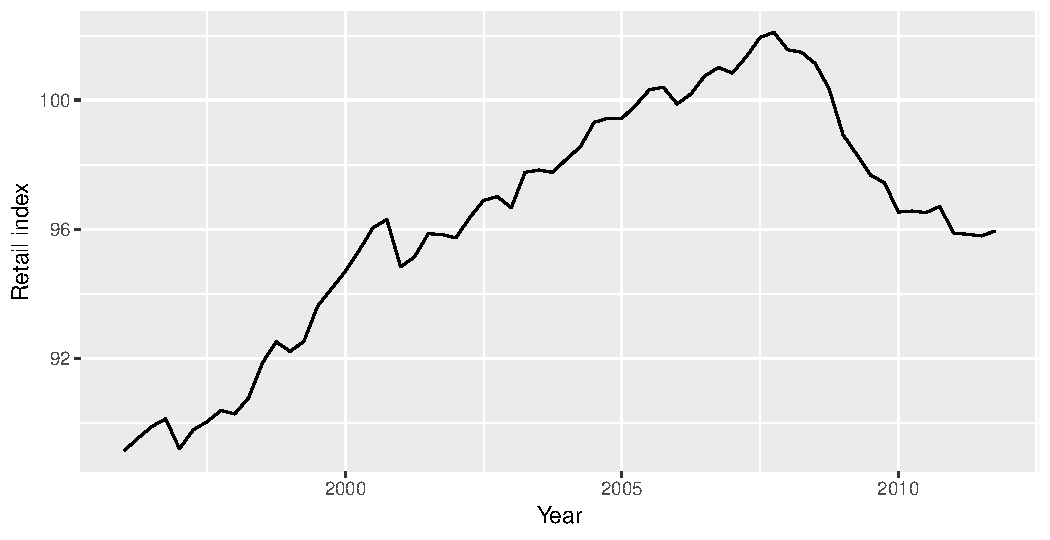
\includegraphics{week_5_arima_files/figure-beamer/unnamed-chunk-42-1.pdf}

\end{frame}

\begin{frame}[fragile]{European quarterly retail trade}

\begin{Shaded}
\begin{Highlighting}[]
\NormalTok{euretail }\OperatorTok\StringTok{ }\KeywordTok{diff}\NormalTok{(}\DataTypeTok{lag=}\DecValTok{4}\NormalTok{) }\OperatorTok\StringTok{ }\KeywordTok{ggtsdisplay}\NormalTok{()}
\end{Highlighting}
\end{Shaded}

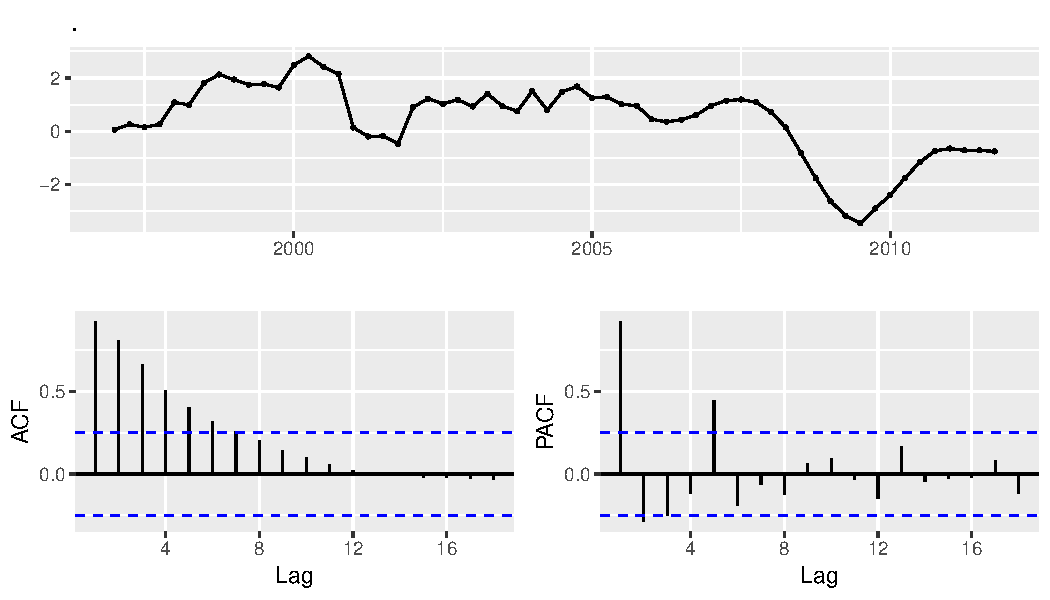
\includegraphics{week_5_arima_files/figure-beamer/unnamed-chunk-43-1.pdf}

\end{frame}

\begin{frame}[fragile]{European quarterly retail trade}

\begin{Shaded}
\begin{Highlighting}[]
\NormalTok{euretail }\OperatorTok\StringTok{ }\KeywordTok{diff}\NormalTok{(}\DataTypeTok{lag=}\DecValTok{4}\NormalTok{) }\OperatorTok\StringTok{ }\KeywordTok{diff}\NormalTok{() }\OperatorTok
\StringTok{  }\KeywordTok{ggtsdisplay}\NormalTok{()}
\end{Highlighting}
\end{Shaded}

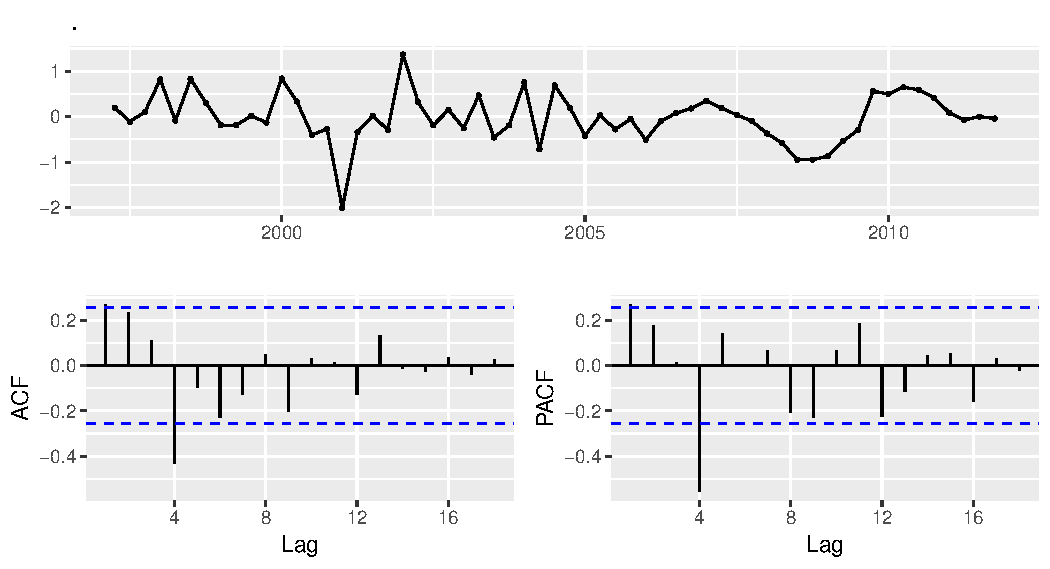
\includegraphics{week_5_arima_files/figure-beamer/unnamed-chunk-44-1.pdf}

\end{frame}

\begin{frame}{European quarterly retail trade}

\begin{itemize}
\tightlist
\item
  \(d=1\) and \(D=1\) seems necessary.
\item
  Significant spike at lag 1 in ACF suggests non-seasonal MA(1)
  component.
\item
  Significant spike at lag 4 in ACF suggests seasonal MA(1) component.
\item
  Initial candidate model: ARIMA(0,1,1)(0,1,1)\(_4\).
\item
  We could also have started with ARIMA(1,1,0)(1,1,0)\(_4\).
\end{itemize}

\end{frame}

\begin{frame}[fragile]{European quarterly retail trade}

\begin{Shaded}
\begin{Highlighting}[]
\NormalTok{fit <-}\StringTok{ }\KeywordTok{Arima}\NormalTok{(euretail, }\DataTypeTok{order=}\KeywordTok{c}\NormalTok{(}\DecValTok{0}\NormalTok{,}\DecValTok{1}\NormalTok{,}\DecValTok{1}\NormalTok{),}
  \DataTypeTok{seasonal=}\KeywordTok{c}\NormalTok{(}\DecValTok{0}\NormalTok{,}\DecValTok{1}\NormalTok{,}\DecValTok{1}\NormalTok{))}
\KeywordTok{checkresiduals}\NormalTok{(fit)}
\end{Highlighting}
\end{Shaded}

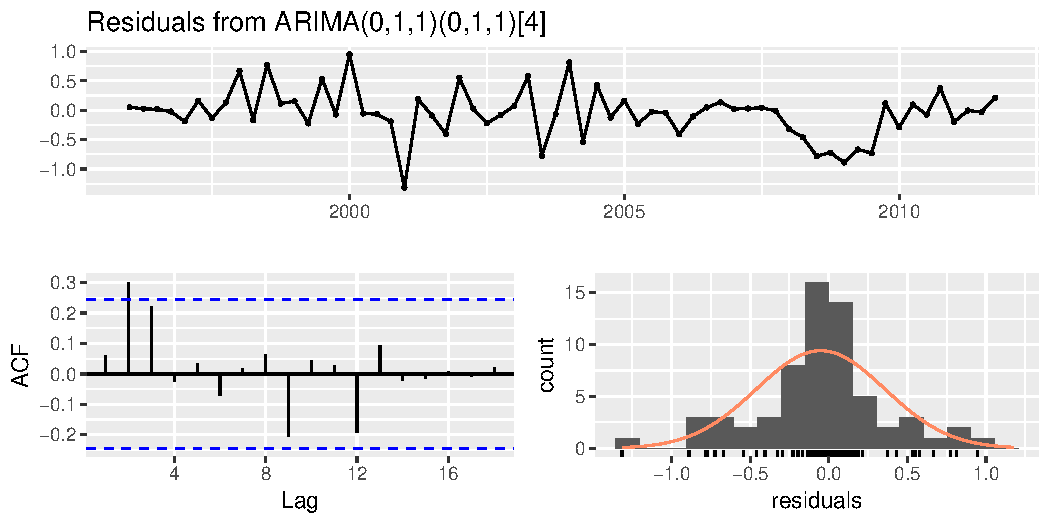
\includegraphics{week_5_arima_files/figure-beamer/unnamed-chunk-45-1.pdf}

\begin{verbatim}
## 
##  Ljung-Box test
## 
## data:  Residuals from ARIMA(0,1,1)(0,1,1)[4]
## Q* = 10.654, df = 6, p-value = 0.09968
## 
## Model df: 2.   Total lags used: 8
\end{verbatim}

\end{frame}

\begin{frame}[fragile]{European quarterly retail trade}

\fontsize{13}{14}\sf

\begin{verbatim}
## 
##  Ljung-Box test
## 
## data:  Residuals from ARIMA(0,1,1)(0,1,1)[4]
## Q* = 10.654, df = 6, p-value = 0.09968
## 
## Model df: 2.   Total lags used: 8
\end{verbatim}

\end{frame}

\begin{frame}[fragile]{European quarterly retail trade}

\begin{itemize}
\tightlist
\item
  ACF and PACF of residuals show significant spikes at lag 2, and maybe
  lag 3.
\item
  AICc of ARIMA(0,1,2)(0,1,1)\(_4\) model is 74.27.
\item
  AICc of ARIMA(0,1,3)(0,1,1)\(_4\) model is 68.39. \pause\vfill
\end{itemize}

\begin{Shaded}
\begin{Highlighting}[]
\NormalTok{fit <-}\StringTok{ }\KeywordTok{Arima}\NormalTok{(euretail, }\DataTypeTok{order=}\KeywordTok{c}\NormalTok{(}\DecValTok{0}\NormalTok{,}\DecValTok{1}\NormalTok{,}\DecValTok{3}\NormalTok{),}
  \DataTypeTok{seasonal=}\KeywordTok{c}\NormalTok{(}\DecValTok{0}\NormalTok{,}\DecValTok{1}\NormalTok{,}\DecValTok{1}\NormalTok{))}
\KeywordTok{checkresiduals}\NormalTok{(fit)}
\end{Highlighting}
\end{Shaded}

\end{frame}

\begin{frame}[fragile]{European quarterly retail trade}

\fontsize{12}{15}\sf

\begin{verbatim}
## Series: euretail 
## ARIMA(0,1,3)(0,1,1)[4] 
## 
## Coefficients:
##          ma1     ma2     ma3     sma1
##       0.2630  0.3694  0.4200  -0.6636
## s.e.  0.1237  0.1255  0.1294   0.1545
## 
## sigma^2 estimated as 0.156:  log likelihood=-28.63
## AIC=67.26   AICc=68.39   BIC=77.65
\end{verbatim}

\end{frame}

\begin{frame}[fragile]{European quarterly retail trade}

\fontsize{13}{15}\sf

\begin{Shaded}
\begin{Highlighting}[]
\KeywordTok{checkresiduals}\NormalTok{(fit)}
\end{Highlighting}
\end{Shaded}

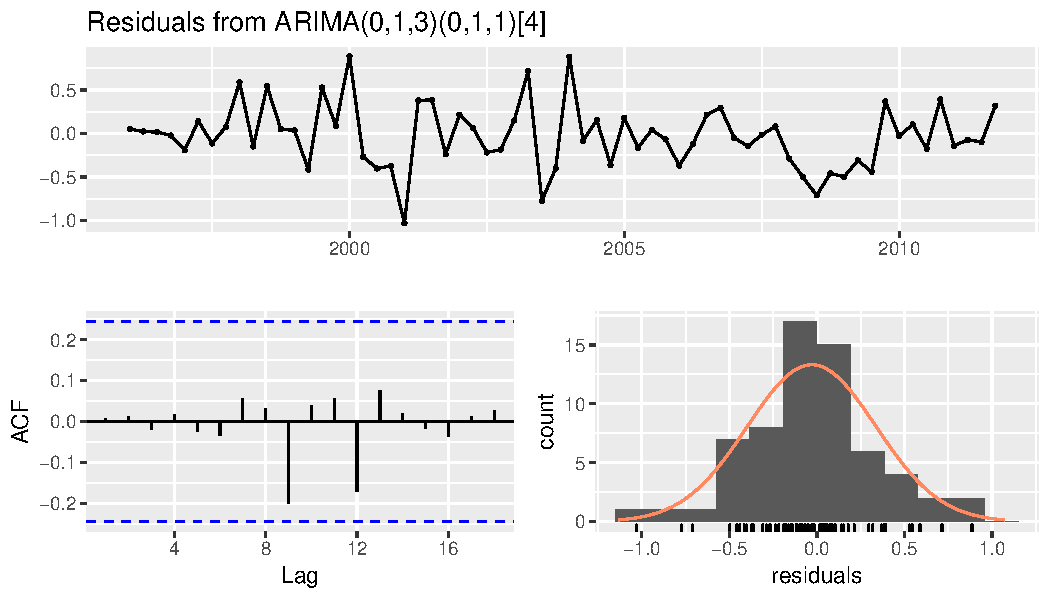
\includegraphics{week_5_arima_files/figure-beamer/unnamed-chunk-49-1.pdf}

\begin{verbatim}
## 
##  Ljung-Box test
## 
## data:  Residuals from ARIMA(0,1,3)(0,1,1)[4]
## Q* = 0.51128, df = 4, p-value = 0.9724
## 
## Model df: 4.   Total lags used: 8
\end{verbatim}

\end{frame}

\begin{frame}[fragile]{European quarterly retail trade}

\fontsize{13}{15}\sf

\begin{verbatim}
## 
##  Ljung-Box test
## 
## data:  Residuals from ARIMA(0,1,3)(0,1,1)[4]
## Q* = 0.51128, df = 4, p-value = 0.9724
## 
## Model df: 4.   Total lags used: 8
\end{verbatim}

\end{frame}

\begin{frame}[fragile]{European quarterly retail trade}

\begin{Shaded}
\begin{Highlighting}[]
\KeywordTok{autoplot}\NormalTok{(}\KeywordTok{forecast}\NormalTok{(fit, }\DataTypeTok{h=}\DecValTok{12}\NormalTok{))}
\end{Highlighting}
\end{Shaded}

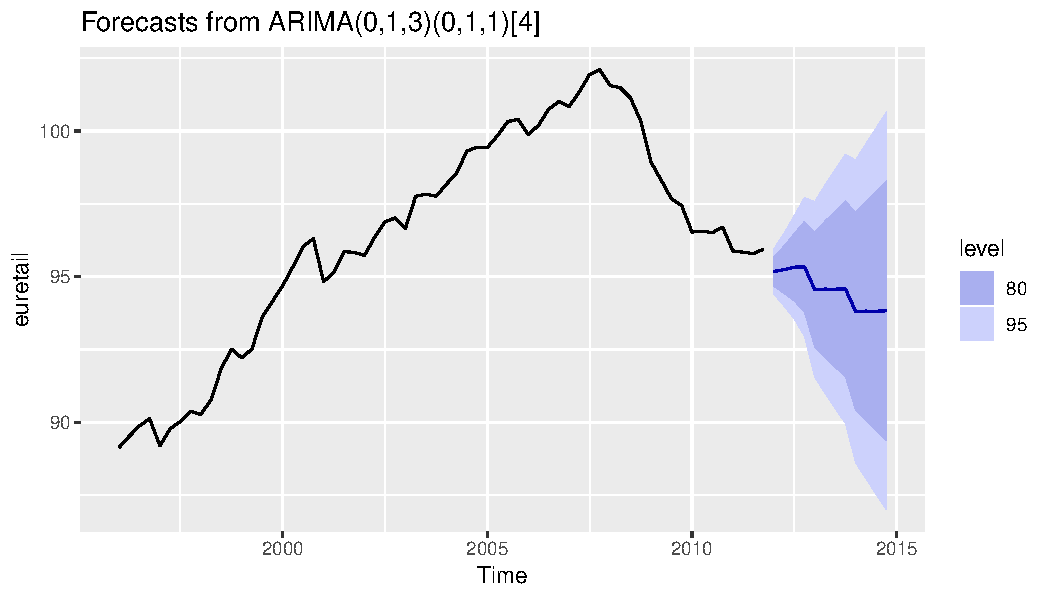
\includegraphics{week_5_arima_files/figure-beamer/unnamed-chunk-51-1.pdf}

\end{frame}

\begin{frame}[fragile]{European quarterly retail trade}

\fontsize{12}{14}\sf

\begin{Shaded}
\begin{Highlighting}[]
\KeywordTok{auto.arima}\NormalTok{(euretail)}
\end{Highlighting}
\end{Shaded}

\begin{verbatim}
## Series: euretail 
## ARIMA(1,1,2)(0,1,1)[4] 
## 
## Coefficients:
##          ar1      ma1     ma2     sma1
##       0.7362  -0.4663  0.2163  -0.8433
## s.e.  0.2243   0.1990  0.2101   0.1876
## 
## sigma^2 estimated as 0.1587:  log likelihood=-29.62
## AIC=69.24   AICc=70.38   BIC=79.63
\end{verbatim}

\end{frame}

\begin{frame}[fragile]{European quarterly retail trade}

\fontsize{12}{14}\sf

\begin{Shaded}
\begin{Highlighting}[]
\KeywordTok{auto.arima}\NormalTok{(euretail, }
  \DataTypeTok{stepwise=}\OtherTok{FALSE}\NormalTok{, }\DataTypeTok{approximation=}\OtherTok{FALSE}\NormalTok{)}
\end{Highlighting}
\end{Shaded}

\begin{verbatim}
## Series: euretail 
## ARIMA(0,1,3)(0,1,1)[4] 
## 
## Coefficients:
##          ma1     ma2     ma3     sma1
##       0.2630  0.3694  0.4200  -0.6636
## s.e.  0.1237  0.1255  0.1294   0.1545
## 
## sigma^2 estimated as 0.156:  log likelihood=-28.63
## AIC=67.26   AICc=68.39   BIC=77.65
\end{verbatim}

\end{frame}

\begin{frame}{Cortecosteroid drug sales}

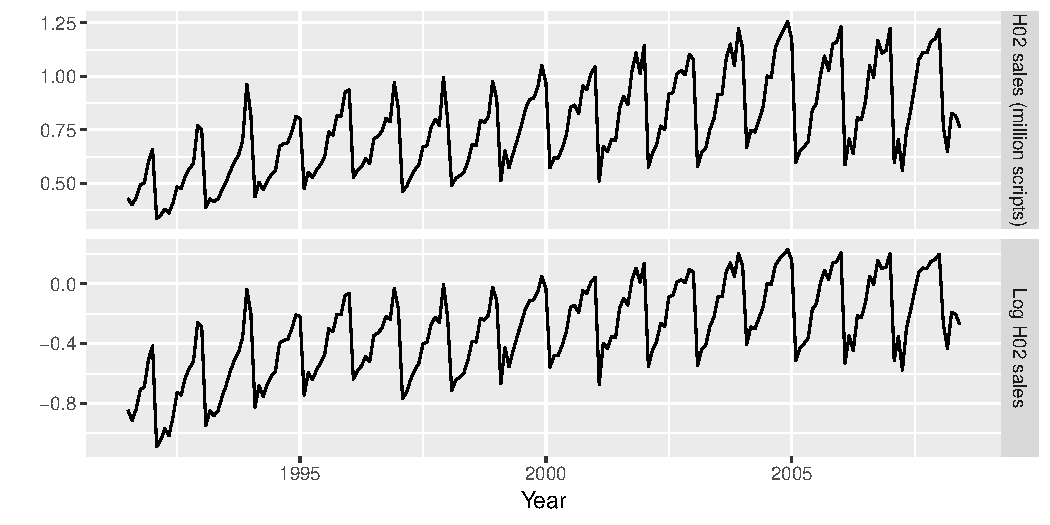
\includegraphics{week_5_arima_files/figure-beamer/h02-1.pdf}

\end{frame}

\begin{frame}{Cortecosteroid drug sales}

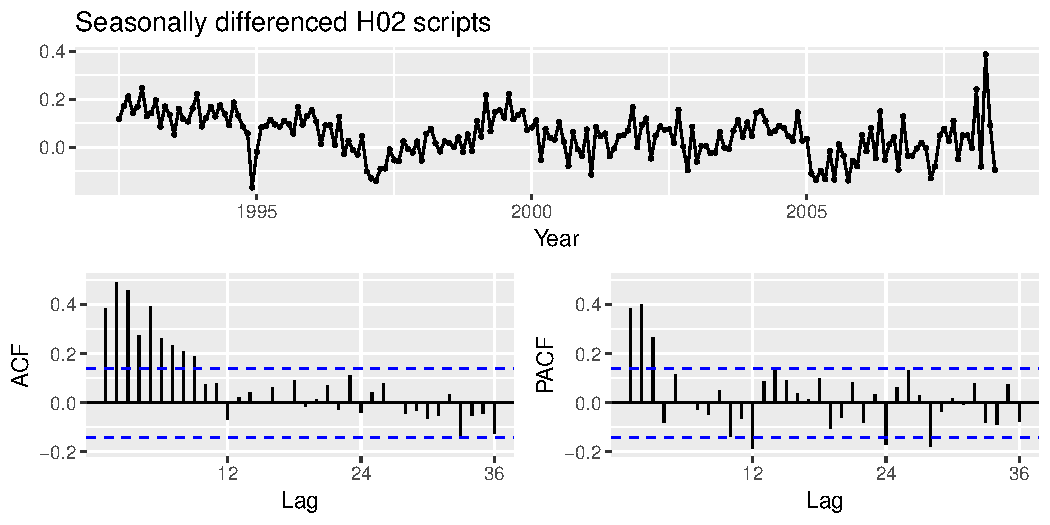
\includegraphics{week_5_arima_files/figure-beamer/h02b-1.pdf}

\end{frame}

\begin{frame}{Cortecosteroid drug sales}

\begin{itemize}
\tightlist
\item
  Choose \(D=1\) and \(d=0\).
\item
  Spikes in PACF at lags 12 and 24 suggest seasonal AR(2) term.
\item
  Spikes in PACF suggests possible non-seasonal AR(3) term.
\item
  Initial candidate model: ARIMA(3,0,0)(2,1,0)\(_{12}\).
\end{itemize}

\end{frame}

\begin{frame}{Cortecosteroid drug sales}

\begin{longtable}[]{@{}cc@{}}
\toprule
Model & AICc\tabularnewline
\midrule
\endhead
ARIMA(3,0,1)(0,1,2)\(_{12}\) & -485.48\tabularnewline
ARIMA(3,0,1)(1,1,1)\(_{12}\) & -484.25\tabularnewline
ARIMA(3,0,1)(0,1,1)\(_{12}\) & -483.67\tabularnewline
ARIMA(3,0,1)(2,1,0)\(_{12}\) & -476.31\tabularnewline
ARIMA(3,0,0)(2,1,0)\(_{12}\) & -475.12\tabularnewline
ARIMA(3,0,2)(2,1,0)\(_{12}\) & -474.88\tabularnewline
ARIMA(3,0,1)(1,1,0)\(_{12}\) & -463.40\tabularnewline
\bottomrule
\end{longtable}

\end{frame}

\begin{frame}[fragile]{Cortecosteroid drug sales}

\fontsize{11}{12}\sf

\begin{Shaded}
\begin{Highlighting}[]
\NormalTok{(fit <-}\StringTok{ }\KeywordTok{Arima}\NormalTok{(h02, }\DataTypeTok{order=}\KeywordTok{c}\NormalTok{(}\DecValTok{3}\NormalTok{,}\DecValTok{0}\NormalTok{,}\DecValTok{1}\NormalTok{), }\DataTypeTok{seasonal=}\KeywordTok{c}\NormalTok{(}\DecValTok{0}\NormalTok{,}\DecValTok{1}\NormalTok{,}\DecValTok{2}\NormalTok{),}
   \DataTypeTok{lambda=}\DecValTok{0}\NormalTok{))}
\end{Highlighting}
\end{Shaded}

\begin{verbatim}
## Series: h02 
## ARIMA(3,0,1)(0,1,2)[12] 
## Box Cox transformation: lambda= 0 
## 
## Coefficients:
##           ar1     ar2     ar3     ma1     sma1     sma2
##       -0.1603  0.5481  0.5678  0.3827  -0.5222  -0.1768
## s.e.   0.1636  0.0878  0.0942  0.1895   0.0861   0.0872
## 
## sigma^2 estimated as 0.004278:  log likelihood=250.04
## AIC=-486.08   AICc=-485.48   BIC=-463.28
\end{verbatim}

\end{frame}

\begin{frame}[fragile]{Cortecosteroid drug sales}

\begin{Shaded}
\begin{Highlighting}[]
\KeywordTok{checkresiduals}\NormalTok{(fit, }\DataTypeTok{lag=}\DecValTok{36}\NormalTok{)}
\end{Highlighting}
\end{Shaded}

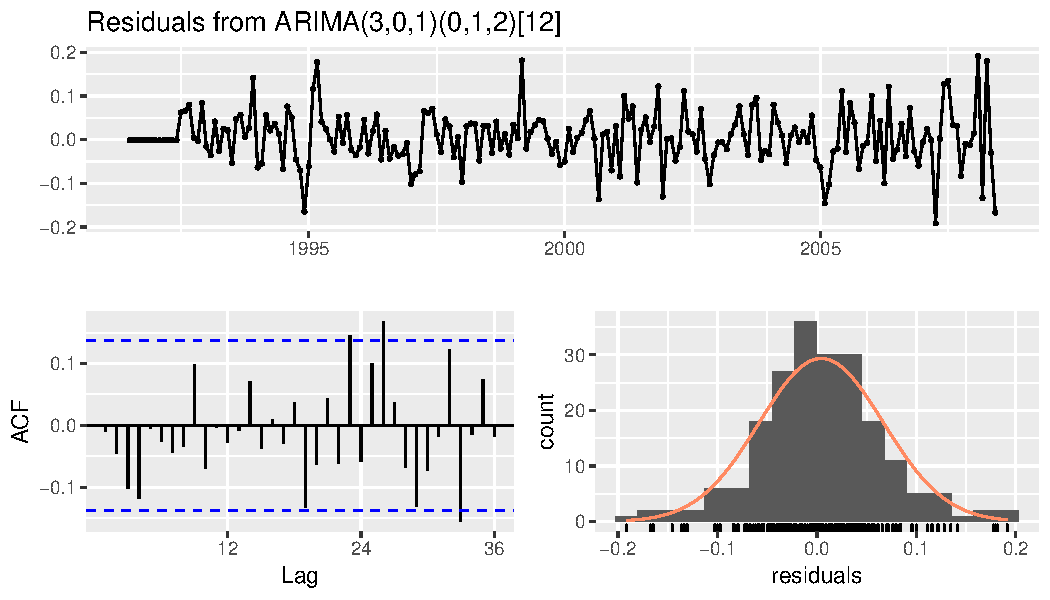
\includegraphics{week_5_arima_files/figure-beamer/h02res-1.pdf}

\begin{verbatim}
## 
##  Ljung-Box test
## 
## data:  Residuals from ARIMA(3,0,1)(0,1,2)[12]
## Q* = 50.712, df = 30, p-value = 0.01045
## 
## Model df: 6.   Total lags used: 36
\end{verbatim}

\end{frame}

\begin{frame}[fragile]{Cortecosteroid drug sales}

\fontsize{11}{15}\sf

\begin{verbatim}
## 
##  Ljung-Box test
## 
## data:  Residuals from ARIMA(3,0,1)(0,1,2)[12]
## Q* = 50.712, df = 30, p-value = 0.01045
## 
## Model df: 6.   Total lags used: 36
\end{verbatim}

\end{frame}

\begin{frame}[fragile]{Cortecosteroid drug sales}

\fontsize{8}{10}\sf

\begin{Shaded}
\begin{Highlighting}[]
\NormalTok{(fit <-}\StringTok{ }\KeywordTok{auto.arima}\NormalTok{(h02, }\DataTypeTok{lambda=}\DecValTok{0}\NormalTok{))}
\end{Highlighting}
\end{Shaded}

\begin{verbatim}
## Series: h02 
## ARIMA(2,1,3)(0,1,1)[12] 
## Box Cox transformation: lambda= 0 
## 
## Coefficients:
##           ar1      ar2     ma1     ma2      ma3     sma1
##       -1.0194  -0.8351  0.1717  0.2578  -0.4206  -0.6528
## s.e.   0.1648   0.1203  0.2079  0.1177   0.1060   0.0657
## 
## sigma^2 estimated as 0.004203:  log likelihood=250.8
## AIC=-487.6   AICc=-486.99   BIC=-464.83
\end{verbatim}

\end{frame}

\begin{frame}[fragile]{Cortecosteroid drug sales}

\fontsize{10}{12}\sf

\begin{Shaded}
\begin{Highlighting}[]
\KeywordTok{checkresiduals}\NormalTok{(fit, }\DataTypeTok{lag=}\DecValTok{36}\NormalTok{)}
\end{Highlighting}
\end{Shaded}

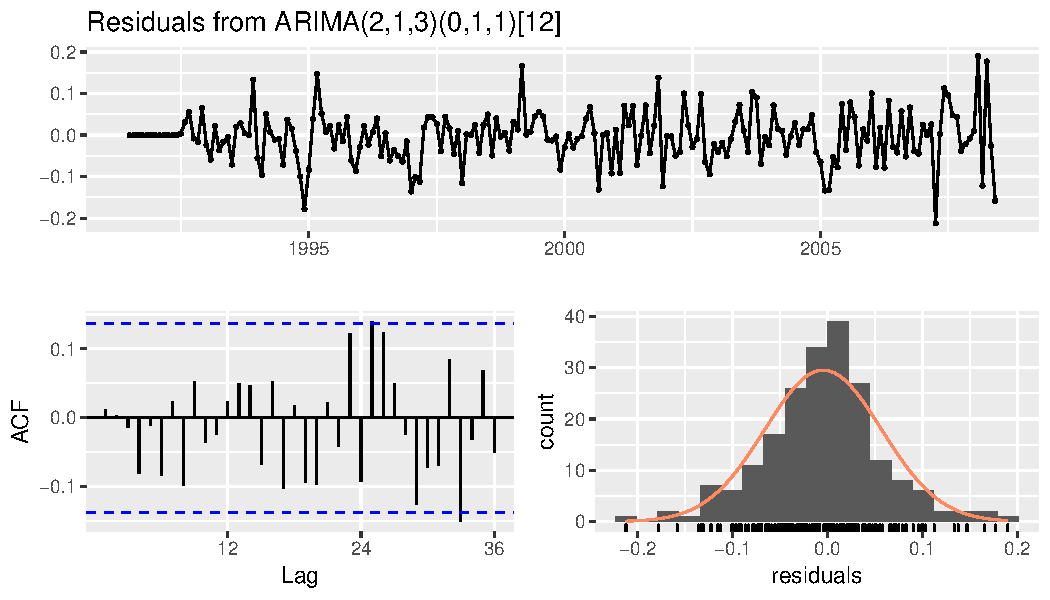
\includegraphics{week_5_arima_files/figure-beamer/unnamed-chunk-53-1.pdf}

\begin{verbatim}
## 
##  Ljung-Box test
## 
## data:  Residuals from ARIMA(2,1,3)(0,1,1)[12]
## Q* = 46.149, df = 30, p-value = 0.03007
## 
## Model df: 6.   Total lags used: 36
\end{verbatim}

\end{frame}

\begin{frame}[fragile]{Cortecosteroid drug sales}

\fontsize{11}{15}\sf

\begin{verbatim}
## 
##  Ljung-Box test
## 
## data:  Residuals from ARIMA(2,1,3)(0,1,1)[12]
## Q* = 46.149, df = 30, p-value = 0.03007
## 
## Model df: 6.   Total lags used: 36
\end{verbatim}

\end{frame}

\begin{frame}[fragile]{Cortecosteroid drug sales}

\fontsize{8}{10}\sf

\begin{Shaded}
\begin{Highlighting}[]
\NormalTok{(fit <-}\StringTok{ }\KeywordTok{auto.arima}\NormalTok{(h02, }\DataTypeTok{lambda=}\DecValTok{0}\NormalTok{, }\DataTypeTok{max.order=}\DecValTok{9}\NormalTok{,}
  \DataTypeTok{stepwise=}\OtherTok{FALSE}\NormalTok{, }\DataTypeTok{approximation=}\OtherTok{FALSE}\NormalTok{))}
\end{Highlighting}
\end{Shaded}

\begin{verbatim}
## Series: h02 
## ARIMA(4,1,1)(2,1,2)[12] 
## Box Cox transformation: lambda= 0 
## 
## Coefficients:
##           ar1     ar2     ar3      ar4      ma1    sar1     sar2     sma1
##       -0.0425  0.2098  0.2017  -0.2273  -0.7424  0.6213  -0.3832  -1.2019
## s.e.   0.2167  0.1813  0.1144   0.0810   0.2074  0.2421   0.1185   0.2491
##         sma2
##       0.4959
## s.e.  0.2135
## 
## sigma^2 estimated as 0.004049:  log likelihood=254.31
## AIC=-488.63   AICc=-487.4   BIC=-456.1
\end{verbatim}

\end{frame}

\begin{frame}[fragile]{Cortecosteroid drug sales}

\fontsize{10}{12}\sf

\begin{Shaded}
\begin{Highlighting}[]
\KeywordTok{checkresiduals}\NormalTok{(fit, }\DataTypeTok{lag=}\DecValTok{36}\NormalTok{)}
\end{Highlighting}
\end{Shaded}

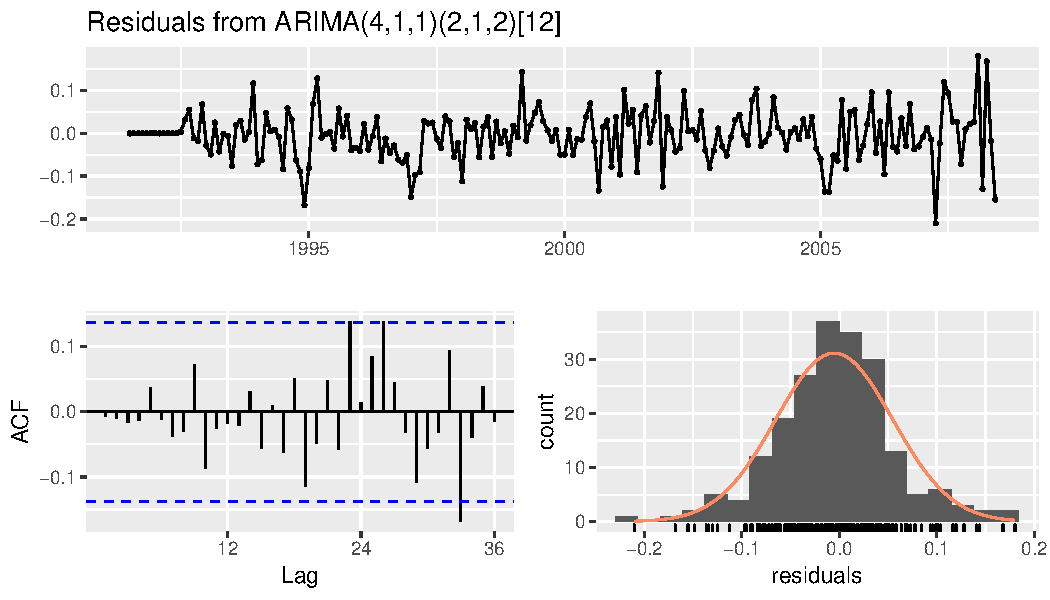
\includegraphics{week_5_arima_files/figure-beamer/unnamed-chunk-55-1.pdf}

\begin{verbatim}
## 
##  Ljung-Box test
## 
## data:  Residuals from ARIMA(4,1,1)(2,1,2)[12]
## Q* = 36.456, df = 27, p-value = 0.1057
## 
## Model df: 9.   Total lags used: 36
\end{verbatim}

\end{frame}

\begin{frame}[fragile]{Cortecosteroid drug sales}

\fontsize{11}{15}\sf

\begin{verbatim}
## 
##  Ljung-Box test
## 
## data:  Residuals from ARIMA(4,1,1)(2,1,2)[12]
## Q* = 36.456, df = 27, p-value = 0.1057
## 
## Model df: 9.   Total lags used: 36
\end{verbatim}

\end{frame}

\begin{frame}[fragile]{Cortecosteroid drug sales}

\fontsize{10}{12}\sf

Training data: July 1991 to June 2006

Test data: July 2006--June 2008

\begin{Shaded}
\begin{Highlighting}[]
\NormalTok{getrmse <-}\StringTok{ }\ControlFlowTok{function}\NormalTok{(x,h,...)}
\NormalTok{\{}
\NormalTok{  train.end <-}\StringTok{ }\KeywordTok{time}\NormalTok{(x)[}\KeywordTok{length}\NormalTok{(x)}\OperatorTok{-}\NormalTok{h]}
\NormalTok{  test.start <-}\StringTok{ }\KeywordTok{time}\NormalTok{(x)[}\KeywordTok{length}\NormalTok{(x)}\OperatorTok{-}\NormalTok{h}\OperatorTok{+}\DecValTok{1}\NormalTok{]}
\NormalTok{  train <-}\StringTok{ }\KeywordTok{window}\NormalTok{(x,}\DataTypeTok{end=}\NormalTok{train.end)}
\NormalTok{  test <-}\StringTok{ }\KeywordTok{window}\NormalTok{(x,}\DataTypeTok{start=}\NormalTok{test.start)}
\NormalTok{  fit <-}\StringTok{ }\KeywordTok{Arima}\NormalTok{(train,...)}
\NormalTok{  fc <-}\StringTok{ }\KeywordTok{forecast}\NormalTok{(fit,}\DataTypeTok{h=}\NormalTok{h)}
  \KeywordTok{return}\NormalTok{(}\KeywordTok{accuracy}\NormalTok{(fc,test)[}\DecValTok{2}\NormalTok{,}\StringTok{"RMSE"}\NormalTok{])}
\NormalTok{\}}
\KeywordTok{getrmse}\NormalTok{(h02,}\DataTypeTok{h=}\DecValTok{24}\NormalTok{,}\DataTypeTok{order=}\KeywordTok{c}\NormalTok{(}\DecValTok{3}\NormalTok{,}\DecValTok{0}\NormalTok{,}\DecValTok{0}\NormalTok{),}\DataTypeTok{seasonal=}\KeywordTok{c}\NormalTok{(}\DecValTok{2}\NormalTok{,}\DecValTok{1}\NormalTok{,}\DecValTok{0}\NormalTok{),}\DataTypeTok{lambda=}\DecValTok{0}\NormalTok{)}
\KeywordTok{getrmse}\NormalTok{(h02,}\DataTypeTok{h=}\DecValTok{24}\NormalTok{,}\DataTypeTok{order=}\KeywordTok{c}\NormalTok{(}\DecValTok{3}\NormalTok{,}\DecValTok{0}\NormalTok{,}\DecValTok{1}\NormalTok{),}\DataTypeTok{seasonal=}\KeywordTok{c}\NormalTok{(}\DecValTok{2}\NormalTok{,}\DecValTok{1}\NormalTok{,}\DecValTok{0}\NormalTok{),}\DataTypeTok{lambda=}\DecValTok{0}\NormalTok{)}
\KeywordTok{getrmse}\NormalTok{(h02,}\DataTypeTok{h=}\DecValTok{24}\NormalTok{,}\DataTypeTok{order=}\KeywordTok{c}\NormalTok{(}\DecValTok{3}\NormalTok{,}\DecValTok{0}\NormalTok{,}\DecValTok{2}\NormalTok{),}\DataTypeTok{seasonal=}\KeywordTok{c}\NormalTok{(}\DecValTok{2}\NormalTok{,}\DecValTok{1}\NormalTok{,}\DecValTok{0}\NormalTok{),}\DataTypeTok{lambda=}\DecValTok{0}\NormalTok{)}
\KeywordTok{getrmse}\NormalTok{(h02,}\DataTypeTok{h=}\DecValTok{24}\NormalTok{,}\DataTypeTok{order=}\KeywordTok{c}\NormalTok{(}\DecValTok{3}\NormalTok{,}\DecValTok{0}\NormalTok{,}\DecValTok{1}\NormalTok{),}\DataTypeTok{seasonal=}\KeywordTok{c}\NormalTok{(}\DecValTok{1}\NormalTok{,}\DecValTok{1}\NormalTok{,}\DecValTok{0}\NormalTok{),}\DataTypeTok{lambda=}\DecValTok{0}\NormalTok{)}
\KeywordTok{getrmse}\NormalTok{(h02,}\DataTypeTok{h=}\DecValTok{24}\NormalTok{,}\DataTypeTok{order=}\KeywordTok{c}\NormalTok{(}\DecValTok{3}\NormalTok{,}\DecValTok{0}\NormalTok{,}\DecValTok{1}\NormalTok{),}\DataTypeTok{seasonal=}\KeywordTok{c}\NormalTok{(}\DecValTok{0}\NormalTok{,}\DecValTok{1}\NormalTok{,}\DecValTok{1}\NormalTok{),}\DataTypeTok{lambda=}\DecValTok{0}\NormalTok{)}
\KeywordTok{getrmse}\NormalTok{(h02,}\DataTypeTok{h=}\DecValTok{24}\NormalTok{,}\DataTypeTok{order=}\KeywordTok{c}\NormalTok{(}\DecValTok{3}\NormalTok{,}\DecValTok{0}\NormalTok{,}\DecValTok{1}\NormalTok{),}\DataTypeTok{seasonal=}\KeywordTok{c}\NormalTok{(}\DecValTok{0}\NormalTok{,}\DecValTok{1}\NormalTok{,}\DecValTok{2}\NormalTok{),}\DataTypeTok{lambda=}\DecValTok{0}\NormalTok{)}
\KeywordTok{getrmse}\NormalTok{(h02,}\DataTypeTok{h=}\DecValTok{24}\NormalTok{,}\DataTypeTok{order=}\KeywordTok{c}\NormalTok{(}\DecValTok{3}\NormalTok{,}\DecValTok{0}\NormalTok{,}\DecValTok{1}\NormalTok{),}\DataTypeTok{seasonal=}\KeywordTok{c}\NormalTok{(}\DecValTok{1}\NormalTok{,}\DecValTok{1}\NormalTok{,}\DecValTok{1}\NormalTok{),}\DataTypeTok{lambda=}\DecValTok{0}\NormalTok{)}
\KeywordTok{getrmse}\NormalTok{(h02,}\DataTypeTok{h=}\DecValTok{24}\NormalTok{,}\DataTypeTok{order=}\KeywordTok{c}\NormalTok{(}\DecValTok{3}\NormalTok{,}\DecValTok{0}\NormalTok{,}\DecValTok{3}\NormalTok{),}\DataTypeTok{seasonal=}\KeywordTok{c}\NormalTok{(}\DecValTok{0}\NormalTok{,}\DecValTok{1}\NormalTok{,}\DecValTok{1}\NormalTok{),}\DataTypeTok{lambda=}\DecValTok{0}\NormalTok{)}
\KeywordTok{getrmse}\NormalTok{(h02,}\DataTypeTok{h=}\DecValTok{24}\NormalTok{,}\DataTypeTok{order=}\KeywordTok{c}\NormalTok{(}\DecValTok{3}\NormalTok{,}\DecValTok{0}\NormalTok{,}\DecValTok{2}\NormalTok{),}\DataTypeTok{seasonal=}\KeywordTok{c}\NormalTok{(}\DecValTok{0}\NormalTok{,}\DecValTok{1}\NormalTok{,}\DecValTok{1}\NormalTok{),}\DataTypeTok{lambda=}\DecValTok{0}\NormalTok{)}
\KeywordTok{getrmse}\NormalTok{(h02,}\DataTypeTok{h=}\DecValTok{24}\NormalTok{,}\DataTypeTok{order=}\KeywordTok{c}\NormalTok{(}\DecValTok{2}\NormalTok{,}\DecValTok{1}\NormalTok{,}\DecValTok{3}\NormalTok{),}\DataTypeTok{seasonal=}\KeywordTok{c}\NormalTok{(}\DecValTok{0}\NormalTok{,}\DecValTok{1}\NormalTok{,}\DecValTok{1}\NormalTok{),}\DataTypeTok{lambda=}\DecValTok{0}\NormalTok{)}
\KeywordTok{getrmse}\NormalTok{(h02,}\DataTypeTok{h=}\DecValTok{24}\NormalTok{,}\DataTypeTok{order=}\KeywordTok{c}\NormalTok{(}\DecValTok{2}\NormalTok{,}\DecValTok{1}\NormalTok{,}\DecValTok{4}\NormalTok{),}\DataTypeTok{seasonal=}\KeywordTok{c}\NormalTok{(}\DecValTok{0}\NormalTok{,}\DecValTok{1}\NormalTok{,}\DecValTok{1}\NormalTok{),}\DataTypeTok{lambda=}\DecValTok{0}\NormalTok{)}
\KeywordTok{getrmse}\NormalTok{(h02,}\DataTypeTok{h=}\DecValTok{24}\NormalTok{,}\DataTypeTok{order=}\KeywordTok{c}\NormalTok{(}\DecValTok{2}\NormalTok{,}\DecValTok{1}\NormalTok{,}\DecValTok{5}\NormalTok{),}\DataTypeTok{seasonal=}\KeywordTok{c}\NormalTok{(}\DecValTok{0}\NormalTok{,}\DecValTok{1}\NormalTok{,}\DecValTok{1}\NormalTok{),}\DataTypeTok{lambda=}\DecValTok{0}\NormalTok{)}
\KeywordTok{getrmse}\NormalTok{(h02,}\DataTypeTok{h=}\DecValTok{24}\NormalTok{,}\DataTypeTok{order=}\KeywordTok{c}\NormalTok{(}\DecValTok{4}\NormalTok{,}\DecValTok{1}\NormalTok{,}\DecValTok{1}\NormalTok{),}\DataTypeTok{seasonal=}\KeywordTok{c}\NormalTok{(}\DecValTok{2}\NormalTok{,}\DecValTok{1}\NormalTok{,}\DecValTok{2}\NormalTok{),}\DataTypeTok{lambda=}\DecValTok{0}\NormalTok{)}
\end{Highlighting}
\end{Shaded}

\end{frame}

\begin{frame}{Cortecosteroid drug sales}

\fontsize{12}{14}\sf

\begin{longtable}[]{@{}lr@{}}
\toprule
Model & RMSE\tabularnewline
\midrule
\endhead
ARIMA(4,1,1)(2,1,2){[}12{]} & 0.0615\tabularnewline
ARIMA(3,0,1)(0,1,2){[}12{]} & 0.0622\tabularnewline
ARIMA(3,0,1)(1,1,1){[}12{]} & 0.0630\tabularnewline
ARIMA(2,1,4)(0,1,1){[}12{]} & 0.0632\tabularnewline
ARIMA(2,1,3)(0,1,1){[}12{]} & 0.0634\tabularnewline
ARIMA(3,0,3)(0,1,1){[}12{]} & 0.0638\tabularnewline
ARIMA(2,1,5)(0,1,1){[}12{]} & 0.0640\tabularnewline
ARIMA(3,0,1)(0,1,1){[}12{]} & 0.0644\tabularnewline
ARIMA(3,0,2)(0,1,1){[}12{]} & 0.0644\tabularnewline
ARIMA(3,0,2)(2,1,0){[}12{]} & 0.0645\tabularnewline
ARIMA(3,0,1)(2,1,0){[}12{]} & 0.0646\tabularnewline
ARIMA(3,0,0)(2,1,0){[}12{]} & 0.0661\tabularnewline
ARIMA(3,0,1)(1,1,0){[}12{]} & 0.0679\tabularnewline
\bottomrule
\end{longtable}

\end{frame}

\begin{frame}{Cortecosteroid drug sales}

\begin{itemize}
\tightlist
\item
  Models with lowest AICc values tend to give slightly better results
  than the other models.
\item
  AICc comparisons must have the same orders of differencing. But RMSE
  test set comparisons can involve any models.
\item
  Use the best model available, even if it does not pass all tests.
\end{itemize}

\end{frame}

\begin{frame}[fragile]{Cortecosteroid drug sales}

\fontsize{11}{14}\sf

\begin{Shaded}
\begin{Highlighting}[]
\NormalTok{fit <-}\StringTok{ }\KeywordTok{Arima}\NormalTok{(h02, }\DataTypeTok{order=}\KeywordTok{c}\NormalTok{(}\DecValTok{3}\NormalTok{,}\DecValTok{0}\NormalTok{,}\DecValTok{1}\NormalTok{), }\DataTypeTok{seasonal=}\KeywordTok{c}\NormalTok{(}\DecValTok{0}\NormalTok{,}\DecValTok{1}\NormalTok{,}\DecValTok{2}\NormalTok{),}
  \DataTypeTok{lambda=}\DecValTok{0}\NormalTok{)}
\KeywordTok{autoplot}\NormalTok{(}\KeywordTok{forecast}\NormalTok{(fit)) }\OperatorTok{+}
\StringTok{  }\KeywordTok{ylab}\NormalTok{(}\StringTok{"H02 sales (million scripts)"}\NormalTok{) }\OperatorTok{+}\StringTok{ }\KeywordTok{xlab}\NormalTok{(}\StringTok{"Year"}\NormalTok{)}
\end{Highlighting}
\end{Shaded}

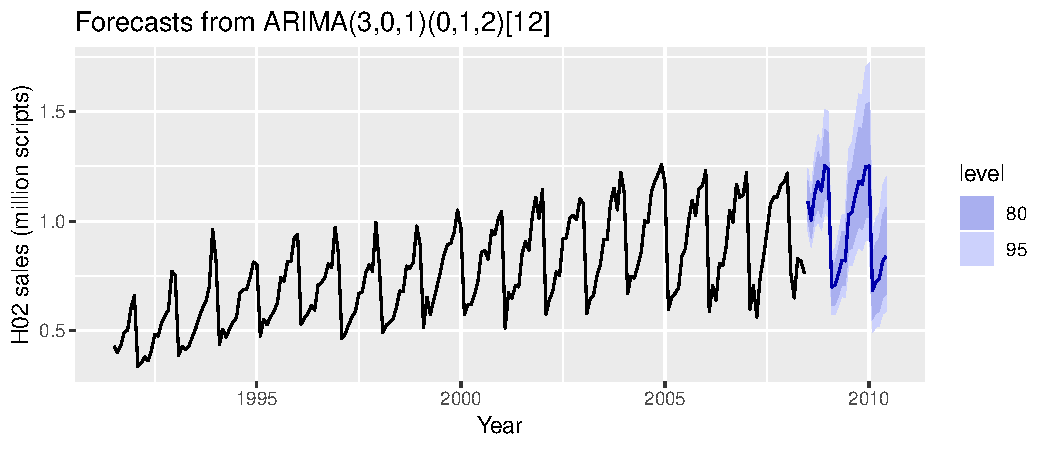
\includegraphics{week_5_arima_files/figure-beamer/h02f-1.pdf}

\end{frame}

\section{ARIMA vs ETS}\label{arima-vs-ets}

\begin{frame}{ARIMA vs ETS}

\begin{itemize}
\item
  Myth that ARIMA models are more general than exponential smoothing.
\item
  Linear exponential smoothing models all special cases of ARIMA models.
\item
  Non-linear exponential smoothing models have no equivalent ARIMA
  counterparts.
\item
  Many ARIMA models have no exponential smoothing counterparts.
\item
  ETS models all non-stationary. Models with seasonality or non-damped
  trend (or both) have two unit roots; all other models have one unit
  \rlap{root.}
\end{itemize}

\vspace*{10cm}

\end{frame}

\begin{frame}{Equivalences}

\fontsize{12}{14}\sf

\begin{longtable}[]{@{}lll@{}}
\toprule
\textbf{ETS model} & \textbf{ARIMA model} &
\textbf{Parameters}\tabularnewline
\midrule
\endhead
ETS(A,N,N) & ARIMA(0,1,1) & \(\theta_1 = \alpha-1\)\tabularnewline
ETS(A,A,N) & ARIMA(0,2,2) & \(\theta_1 = \alpha+\beta-2\)\tabularnewline
& & \(\theta_2 = 1-\alpha\)\tabularnewline
ETS(A,A,N) & ARIMA(1,1,2) & \(\phi_1=\phi\)\tabularnewline
& & \(\theta_1 = \alpha+\phi\beta-1-\phi\)\tabularnewline
& & \(\theta_2 = (1-\alpha)\phi\)\tabularnewline
ETS(A,N,A) & ARIMA(0,0,\(m\))(0,1,0)\(_m\) &\tabularnewline
ETS(A,A,A) & ARIMA(0,1,\(m+1\))(0,1,0)\(_m\) &\tabularnewline
ETS(A,A,A) & ARIMA(1,0,\(m+1\))(0,1,0)\(_m\) &\tabularnewline
\bottomrule
\end{longtable}

\end{frame}

\begin{frame}[fragile]{Your turn}

\fontsize{13}{13}\sf

For the \texttt{condmilk} series:

\begin{itemize}
\tightlist
\item
  Do the data need transforming? If so, find a suitable transformation.
\item
  Are the data stationary? If not, find an appropriate differencing
  which yields stationary data.
\item
  Identify a couple of ARIMA models that might be useful in describing
  the time series.
\item
  Which of your models is the best according to their AIC values?
\item
  Estimate the parameters of your best model and do diagnostic testing
  on the residuals. Do the residuals resemble white noise? If not, try
  to find another ARIMA model which fits better.
\item
  Forecast the next 24 months of data using your preferred model.
\item
  Compare the forecasts obtained using \texttt{ets()}.
\end{itemize}

\end{frame}

\end{document}
